% Created 2019-04-15 Mon 07:05
% Intended LaTeX compiler: pdflatex
\documentclass[dvipdfmx,bigger,aspectratio=169]{beamer}
\usepackage[utf8]{inputenc}
\usepackage[T1]{fontenc}
\usepackage{graphicx}
\usepackage{grffile}
\usepackage{longtable}
\usepackage{wrapfig}
\usepackage{rotating}
\usepackage[normalem]{ulem}
\usepackage{amsmath}
\usepackage{textcomp}
\usepackage{amssymb}
\usepackage{capt-of}
\usepackage{hyperref}
%% No navigation bar
\setbeamertemplate{navigation symbols}{}
%% Page number with current/total format
\setbeamerfont{page number in head/foot}{size=\scriptsize}
\setbeamertemplate{footline}[frame number]
\setbeamertemplate{frametitle}[default][center]
\setbeamersize{text margin left=5mm,text margin right=5mm}
%% With item labels
\setbeamertemplate{bibliography item}{\insertbiblabel}
%% Without item labels
%% \setbeamertemplate{bibliography item}{}
%% Math
\usepackage{amsmath}
\usepackage{amssymb}
\usepackage{wasysym}
%% Allow new page within align
\allowdisplaybreaks
\usepackage{cancel}
%% Code
\usepackage{listings}
\usepackage{courier}
\lstset{basicstyle=\footnotesize\ttfamily, breaklines=true, frame=single}
\usepackage[cache=false]{minted}
\usemintedstyle{vs}
%% Graphics
\usepackage{graphicx}
\usepackage{grffile}
%% DAG
\usepackage{tikz}
\usetikzlibrary{positioning,shapes.geometric}
%% Allow URL embedding
\usepackage{url}
%% Do not count backup slides.
%% https://tex.stackexchange.com/questions/70448/dont-count-backup-slides
\usepackage{appendixnumberbeamer}
%% https://www.sharelatex.com/learn/Hyperlinks
\usepackage{hyperref}
\hypersetup{
colorlinks = true,
linkcolor= blue
}
\usepackage{fontawesome}
%% Include convenient commands.
\input{\string~/.emacs.d/misc/GrandMacros}
\usetheme{default}
\author{Kazuki Yoshida \\ \\ Division of Rheumatology, Immunology and Allergy \\ Brigham and Women's Hospital \& Harvard Medical School \\ \faTwitter @kaz\_yos \faGithub kaz-yos \faEnvelope kazukiyoshida@mail.harvard.edu}
\date{2019-05-20\\ Mini-Statistics Camp Series \\ BWH Bioinformatics Club \\}
\title{What is the \\ Expectation Maximization \\ (EM) Algorithm? \\}
\hypersetup{
 pdfauthor={Kazuki Yoshida \\ \\ Division of Rheumatology, Immunology and Allergy \\ Brigham and Women's Hospital \& Harvard Medical School \\ \faTwitter @kaz\_yos \faGithub kaz-yos \faEnvelope kazukiyoshida@mail.harvard.edu},
 pdftitle={What is the \\ Expectation Maximization \\ (EM) Algorithm? \\},
 pdfkeywords={},
 pdfsubject={},
 pdfcreator={Emacs 27.0.50 (Org mode 9.2.3)}, 
 pdflang={English}}
\begin{document}

\maketitle
\section{Opening}
\label{sec:orgb609150}


\section{Introduction}
\label{sec:org0b512a1}
\begin{frame}[label={sec:orgff30f97}]{Article Covered}
\begin{itemize}
\item Do and Batzoglou. "What is the expectation maximization algorith?" Nat. Biotechnol. 2008;26:897. \cite{doWhatExpectationMaximization2008} \href{https://www.cmi.ac.in/\~madhavan/courses/dmml2019jan/literature/EM\_algorithm\_2coin\_example.pdf}{pdf1} \href{http://www.utdallas.edu/\~prr105020/biol6385/2019/lecture/lecture\_4\_em\_paper.pdf}{pdf2}
\end{itemize}
\begin{center}
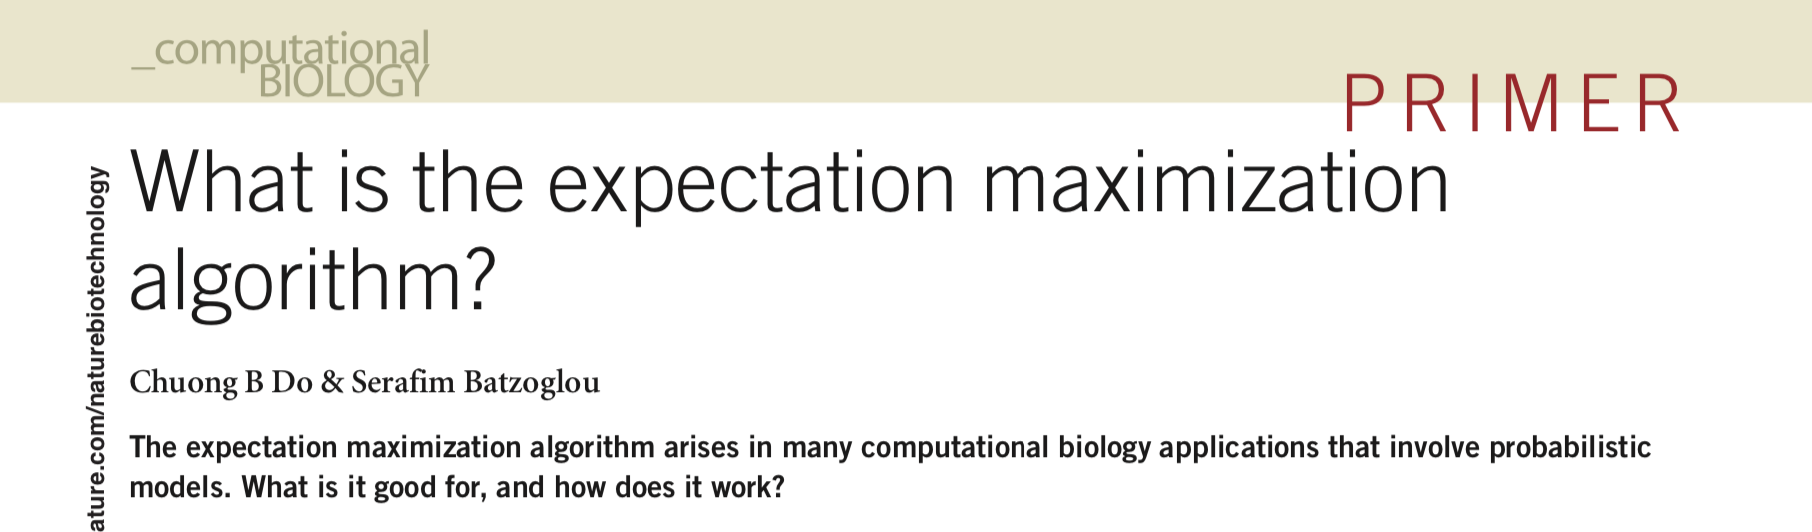
\includegraphics[page=1,keepaspectratio,width=0.8\textwidth]{./source/em_algo.png}
\end{center}
\footnotesize
To be presented as a part of the Mini Statistics Camp 2019 hosted by the \href{http://bioinformatics.bwh.harvard.edu}{BWH/HMS Bioinformatics Club}. The slides contain the corresponding Bayesian inference using the \hyperlink{sec:org536f30f}{Data Augmentation} method and \hyperlink{sec:org6e2589f}{Stan}.
\end{frame}

\begin{frame}[label={sec:orgf029e75}]{Introduction}
\begin{itemize}
\item Probabilistic models, such as hidden Markov models and Bayesian networks, are commonly used to model biological data.
\end{itemize}


\begin{itemize}
\item Often, the only data available for training probabilistic models are incomplete, requiring special handling.
\end{itemize}


\begin{itemize}
\item The Expectation-Maximization (EM) algorithm enables parameter estimation in probabilistic models with incomplete data.
\end{itemize}
\end{frame}


\begin{frame}[label={sec:org288e94e}]{Incomplete data}
\begin{columns}
\begin{column}{0.45\columnwidth}
\begin{itemize}
\item Incomplete data encompass:
\begin{itemize}
\item Typical missing data
\item Latent class (entirely unobserved class assignment)
\end{itemize}
\end{itemize}
\end{column}

\begin{column}{0.45\columnwidth}
\begin{center}
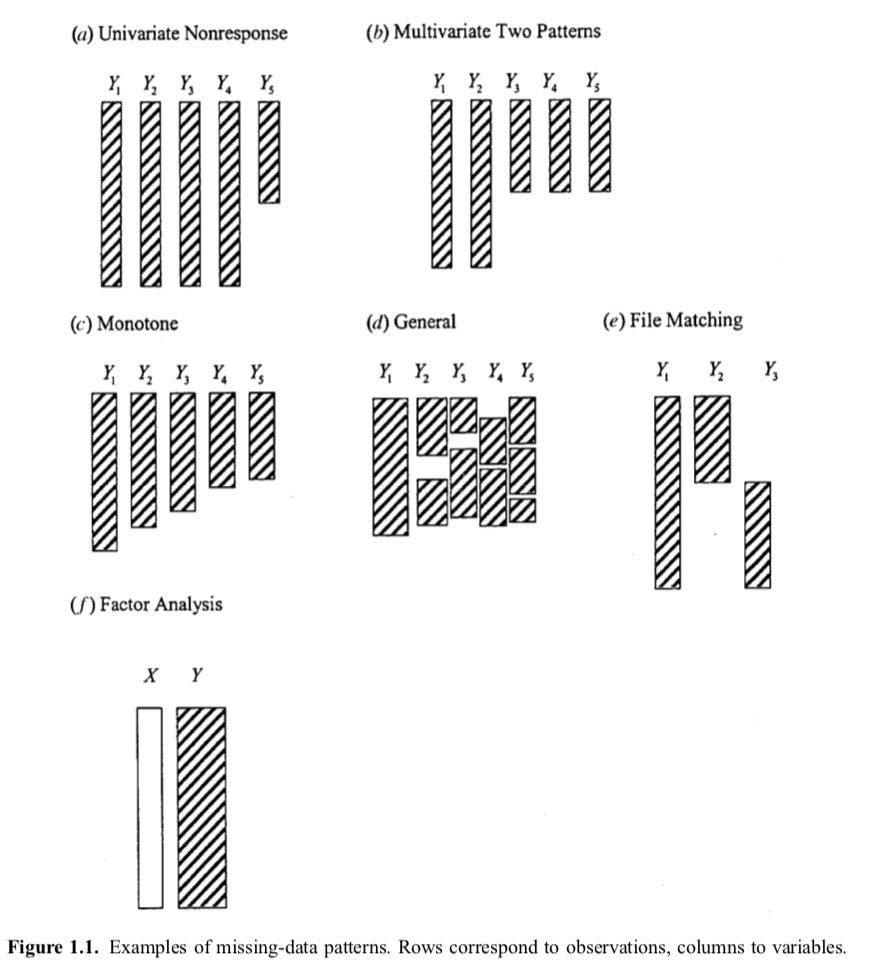
\includegraphics[page=1,keepaspectratio,width=\textwidth,height=0.75\textheight]{./source/missing_patterns.png}
\end{center}
\scriptsize \cite{littleStatisticalAnalysisMissing2002} \normalsize
\end{column}
\end{columns}
\end{frame}

\section{Experiment Setup}
\label{sec:org34bc136}
\begin{frame}[label={sec:orgf30ec00}]{A Coin-Flipping Experiment}
\begin{itemize}
\item Two coins \(A\) (0) and \(B\) (1) with unknown head probabilities \((\theta_{0},\theta_{1})\)
\item Repeat 5 times
\begin{enumerate}
\item Randomly pick either coin with equal probability and record
\item Toss 10 times and record the number of heads
\end{enumerate}
\end{itemize}
\begin{center}
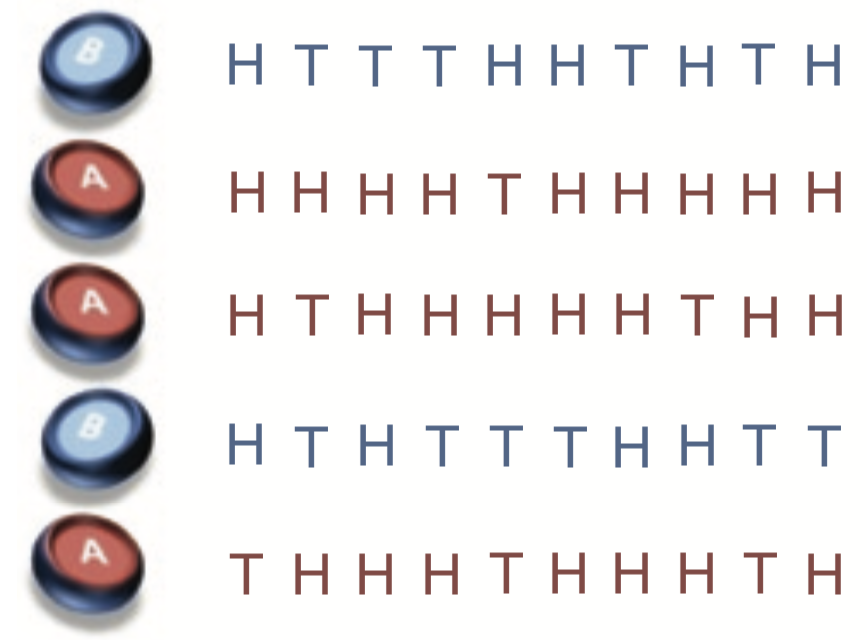
\includegraphics[page=1,keepaspectratio,height=0.5\textheight]{./source/experiment_data.png}
\end{center}
\end{frame}

\begin{frame}[label={sec:orgfe53169}]{A Coin-Flipping Experiment (More Formal)}
\begin{itemize}
\item Two coins \(A\) (0) and \(B\) (1) with unknown head probabilities \((\theta_{0},\theta_{1})\)
\item For \(i = 1, \dots, 5\)
\begin{enumerate}
\item Draw \(Z_{i} \sim \text{Bernoulli}(p = 0.5), Z_{i} \in \left\{ 0,1 \right\}\)
\item Draw \(X_{i} | Z_{i} \sim \text{Binomial}(n = 10, p = \theta_{Z_{i}}), X_{i} \in \left\{ 0, \dots, 10 \right\}\)
\end{enumerate}
\end{itemize}
\begin{center}
\begin{tabular}{rrr}
Index & Coin & Heads\\
\(i\) & \(Z_{i}\) & \(X_{i}\)\\
\hline
1 & 1 & 5\\
2 & 0 & 9\\
3 & 0 & 8\\
4 & 1 & 4\\
5 & 0 & 7\\
\end{tabular}
\end{center}
\begin{itemize}
\item Note that you only need the number of heads (\href{https://www.statisticshowto.datasciencecentral.com/sufficient-statistic/}{sufficient statistic}), not the entire sequence.
\end{itemize}
\end{frame}

\section{Complete-Data Case}
\label{sec:org1e7b404}
\begin{frame}[label={sec:orgf18743e}]{Complete-Data Maximum Likelihood}
\begin{itemize}
\item If we observe both the coin identity \(Z_{i}\) and heads \(X_{i}\), the MLE is the total heads / total tosses for each coin.
\item Here we introduce a very redundant expanded table for later reuse.
\end{itemize}
\footnotesize
\begin{center}
\begin{tabular}{r|l|rr|r|ll|}
Index & Coin & Prob. Coin A & Prob. Coin B & Heads & Heads Coin A & Heads Coin B\\
\(i\) & \(Z_{i}\) & \(E[(1-Z_{i})\vert Z_{i},X_{i}]\) & \(E[Z_{i}\vert Z_{i},X_{i}]\) & \(X_{i}\) & \(E[(1-Z_{i}) X_{i} \vert Z_{i},X_{i}]\) & \(E[Z_{i} X_{i} \vert Z_{i},X_{i}]\)\\
\hline
1 & 1 (B) & 0 & 1 & 5 & 0 \texttimes{} 5 & 1 \texttimes{} 5\\
2 & 0 (A) & 1 & 0 & 9 & 1 \texttimes{} 9 & 0 \texttimes{} 9\\
3 & 0 (A) & 1 & 0 & 8 & 1 \texttimes{} 8 & 0 \texttimes{} 8\\
4 & 1 (B) & 0 & 1 & 4 & 0 \texttimes{} 4 & 1 \texttimes{} 4\\
5 & 0 (A) & 1 & 0 & 7 & 1 \texttimes{} 7 & 0 \texttimes{} 7\\
\hline
Sum &  & 3 & 2 & 33 & 24 & 9\\
\end{tabular}
\end{center}
\begin{itemize}
\item MLE: \(\thetahat_{0} = 24 / (3 \times 10) = 0.80\); \(\thetahat_{1} = 9 / (2 \times 10) = 0.45\)
\end{itemize}
\end{frame}

\begin{frame}[allowframebreaks,label=,t]{Complete-Data Likelihood and Log Likelihood}
\begin{align*}
  L(\btheta | \bz,\bx)
  &= \prod^{5}_{i=1} p(z_{i},x_{i} | \btheta)\\
  &= \prod^{5}_{i=1} p(x_{i} | z_{i}, \btheta) p(z_{i} | \btheta)\\
  &= \prod^{5}_{i=1} p(x_{i} | z_{i}, \btheta) p(z_{i})\\
  &= \prod^{5}_{i=1} p(x_{i} | z_{i}, \btheta) (0.5)\\
  &\propto \prod^{5}_{i=1}
    \left[ \theta_{0}^{x_{i}}(1-\theta_{0})^{10-x_{i}} \right]^{1-z_{i}}
    \left[ \theta_{1}^{x_{i}}(1-\theta_{1})^{10-x_{i}} \right]^{z_{i}}\\
  \log L(\btheta | \bz,\bx)
  &\propto \sum^{5}_{i=1}
    \left\{
    (1-z_{i}) \log \left[ \theta_{0}^{x_{i}}(1-\theta_{0})^{10-x_{i}} \right] +
    z_{i} \log \left[ \theta_{1}^{x_{i}}(1-\theta_{1})^{10-x_{i}} \right]
    \right\}\\
  &= \sum^{5}_{i=1}
    \left\{
    (1-z_{i}) \left[ x_{i}\log\theta_{0} + (10-x_{i})\log(1-\theta_{0})\right]
    \right.\\
  &~~~~~~~~~ \left.
    + z_{i} \left[ x_{i}\log\theta_{1} + (10-x_{i})\log(1-\theta_{1})\right]
    \right\}
\end{align*}
\begin{itemize}
\item We can take partial derivatives with respect to \(\theta_{0}\) and \(\theta_{1}\) and set them to zero to solve for MLE, which gives us heads/tosses for each coin.
\end{itemize}
\end{frame}

\begin{frame}[label={sec:org01c78bd}]{Complete-Data Likelihood Visualization}
\begin{columns}
\begin{column}{0.50\columnwidth}
\begin{itemize}
\item Here the complete-data likelihood function is convex.
\item There is a unique maximum with an analytical solution (coin-specific heads/tosses).
\end{itemize}
\end{column}

\begin{column}{0.50\columnwidth}
\scriptsize
\begin{center}
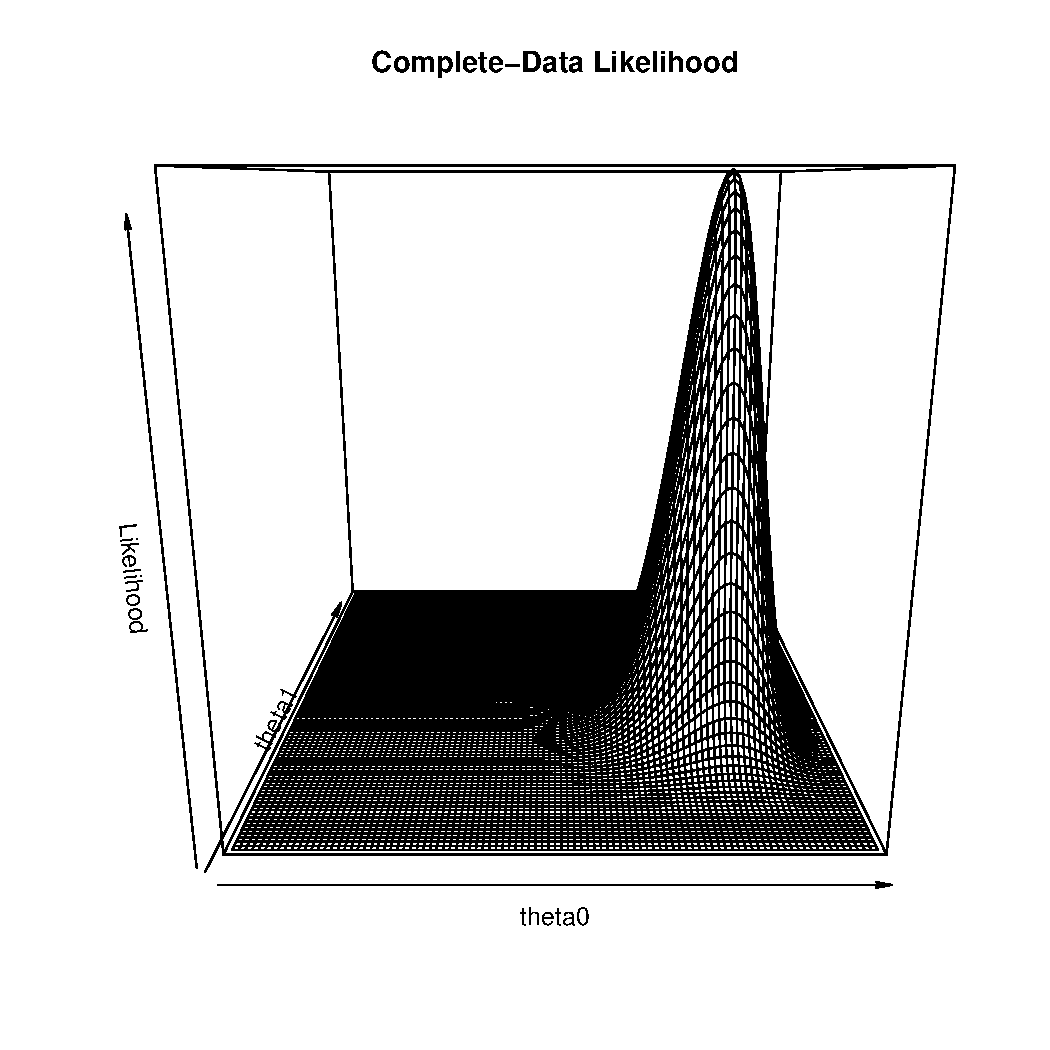
\includegraphics[page=1,keepaspectratio,width=\textwidth,height=\textheight]{./source/likelihood.pdf}
\end{center}
\normalsize
\end{column}
\end{columns}
\end{frame}

\section{Experiment Setup (Incomplete Data)}
\label{sec:orgde83220}
\begin{frame}[label={sec:orge40549a}]{A Contrived Coin-Flipping Experiment}
\begin{itemize}
\item Two identical-looking coins with unknown head probabilities
\item Repeat 5 times
\begin{enumerate}
\item You are randomly given either coin, but you do not know which.
\item You toss 10 times, record the number of heads, and return the coin.
\end{enumerate}
\end{itemize}
\begin{center}
\begin{tabular}{rlr}
Index & Coin & Heads\\
\(i\) & \(Z_{i}\) & \(X_{i}\)\\
\hline
1 & ? & 5\\
2 & ? & 9\\
3 & ? & 8\\
4 & ? & 4\\
5 & ? & 7\\
\end{tabular}
\end{center}
\begin{itemize}
\item Can we still estimate the two unknown head probabilities given this incomplete data?
\end{itemize}
\end{frame}

\begin{frame}[label={sec:org973aae4}]{A Contrived Coin-Flipping Experiment (More Formal)}
\begin{itemize}
\item Two identical-looking coins with unknown head probabilities \((\theta_{0},\theta_{1})\) (index arbitrary)
\item For \(i = 1, \dots, 5\)
\begin{enumerate}
\item Draw \emph{latent} \(Z_{i} \sim \text{Bernoulli}(p = 0.5), Z_{i} \in \left\{ 0,1 \right\}\)
\item Draw \(X_{i} | Z_{i} \sim \text{Binomial}(n = 10, p = \theta_{Z_{i}}), X_{i} \in \left\{ 0, \dots, 10 \right\}\)
\end{enumerate}
\end{itemize}
\begin{center}
\begin{tabular}{rlr}
Index & Coin & Heads\\
\(i\) & \(Z_{i}\) & \(X_{i}\)\\
\hline
1 & ? & 5\\
2 & ? & 9\\
3 & ? & 8\\
4 & ? & 4\\
5 & ? & 7\\
\end{tabular}
\end{center}
\end{frame}

\begin{frame}[label={sec:orgbe50256}]{How Do We Approach Incomplete Data}
\begin{itemize}
\item Now we cannot compute the proportion of heads among tosses for each coin.
\item However, one possible iterative scheme is:
\begin{itemize}
\item Assign some initial guess for parameters
\item Guess coin identities given data and assuming these parameter values
\item Perform MLE given data and assuming coin identities
\end{itemize}
\item The Expectation-Maximization (EM) Algorithm \cite{dempsterMaximumLikelihoodIncomplete1977} is a refinement of this idea for MLE.
\item The Data Augmentation Method \cite{tannerCalculationPosteriorDistributions1987} is another type of refinement for Bayesian estimation.
\end{itemize}
\end{frame}

\section{EM Algorithm}
\label{sec:org21fd39e}
\begin{frame}[label={sec:org2db269e}]{}
\begin{center}
\resizebox{\linewidth}{!}{Expectation-Maximization Algorithm}
\end{center}
\end{frame}

\begin{frame}[label={sec:org066ec30}]{EM Algorithm to the Rescue}
\begin{itemize}
\item The Expectation-Maximization (EM) Algorithm \cite{dempsterMaximumLikelihoodIncomplete1977}
\item After random initialization of parameters, two steps alternates until convergence to an MLE.
\item Steps repeated
\begin{enumerate}
\item E-Step (compute Expected sufficient statistics):
\begin{itemize}
\item Estimate probabilities of latent states given current parameters (coin identity probabilities)
\item Obtain expected sufficient statistics (weighted head counts distributed across coins)
\end{itemize}
\item M-Step (Maximize expected log-likelihood):
\begin{itemize}
\item Obtain MLE of parameters given expected sufficient statistics and update parameters
\end{itemize}
\end{enumerate}
\item By using weighted training data, the EM algorithm accounts for the confidence in the guessed latent state.
\end{itemize}
\end{frame}

\begin{frame}[label={sec:orgd58c90d}]{}
\begin{center}
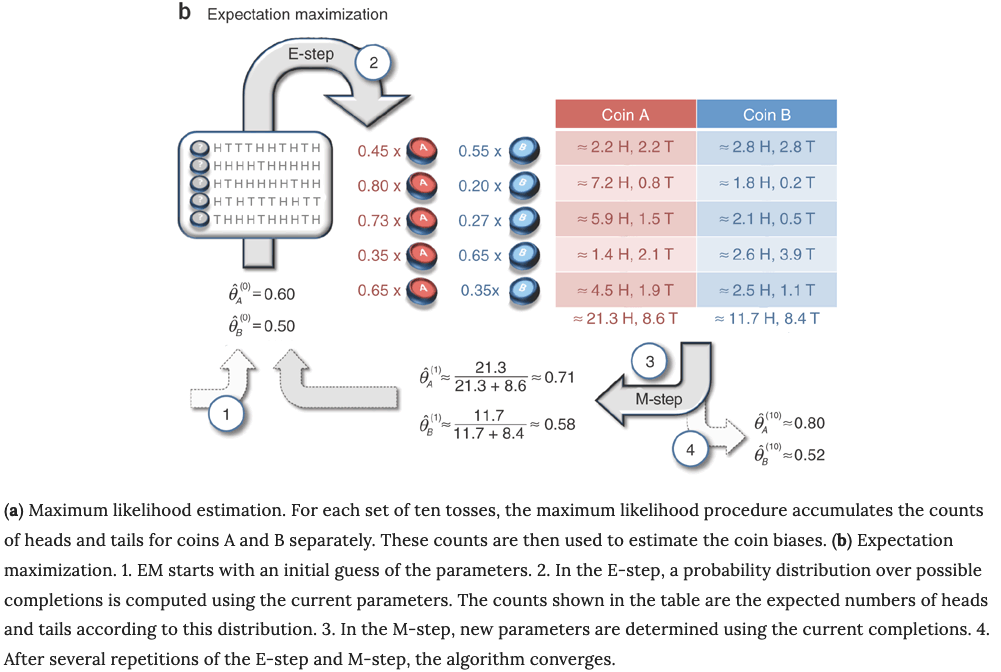
\includegraphics[page=1,keepaspectratio,width=\textwidth,height=\textheight]{./source/em_figure.png}
\end{center}
\end{frame}


\begin{frame}[label={sec:org6b47dd5}]{Parameter Initialization}
\begin{itemize}
\item Randomly initialize the parameters
\begin{itemize}
\item \(\thetahat_{0}^{(0)} := 0.6\)
\item \(\thetahat_{1}^{(0)} := 0.5\)
\end{itemize}
\end{itemize}
\end{frame}

\begin{frame}[fragile,allowframebreaks,label=,t]{E-Step (0)}
 \begin{itemize}
\item Current parameters: \(\thetahat_{0}^{(0)} = 0.6, \thetahat_{1}^{(0)} = 0.5\)
\end{itemize}
\footnotesize
\begin{center}
\begin{tabular}{r|l|ll|r|ll|}
Index & Coin & Prob. Coin A & Prob. Coin B & Heads & Heads Coin A & Heads Coin B\\
\(i\) & \(Z_{i}\) & \(E[(1-Z_{i})\vert X_{i}]\) & \(E[Z_{i}\vert X_{i}]\) & \(X_{i}\) & \(E[(1-Z_{i}) X_{i} \vert X_{i}]\) & \(E[Z_{i} X_{i} \vert X_{i}]\)\\
\hline
1 & ? & ? & ? & 5 & ? \texttimes{} 5 & ? \texttimes{} 5\\
2 & ? & ? & ? & 9 & ? \texttimes{} 9 & ? \texttimes{} 9\\
3 & ? & ? & ? & 8 & ? \texttimes{} 8 & ? \texttimes{} 8\\
4 & ? & ? & ? & 4 & ? \texttimes{} 4 & ? \texttimes{} 4\\
5 & ? & ? & ? & 7 & ? \texttimes{} 7 & ? \texttimes{} 7\\
\hline
Sum &  & ? & ? & 33 & ? & ?\\
\end{tabular}
\end{center}
\normalsize
\begin{itemize}
\item First, we need coin probabilities for each \(i\) given the current parameter values \(\bthetahat^{(0)}\).
\item We will focus on \(E_{\bthetahat^{(0)}}[Z_{i} | X_{i} = x_{i}]\), the probability of Coin B given the number of heads observed and current parameters.
\end{itemize}

\newpage
\begin{itemize}
\item Probability of Coin B given the number of heads observed and current parameters:
\end{itemize}
\footnotesize
\begin{align*}
  E_{\bthetahat^{(0)}}[Z_{i} | X_{i} = x_{i}] &= P_{\bthetahat^{(0)}}[Z_{i} = 1 | X_{i} = x_{i}]\\
  &~~~\text{Bayes rule}\\
  &= \frac{P_{\bthetahat^{(0)}}[X_{i} = x_{i} | Z_{i} = 1] P_{\bthetahat^{(0)}}[Z_{i} = 1]}
          {\sum\limits^{1}_{z=0} P_{\bthetahat^{(0)}}[X_{i} = x_{i} | Z_{i} = z] P_{\bthetahat^{(0)}}[Z_{i} = z]}\\
  &~~~\text{Coin choice probability = 0.5}\\
  &= \frac{P_{\bthetahat^{(0)}}[X_{i} = x_{i} | Z_{i} = 1] (0.5)}
          {\sum\limits^{1}_{z=0} P_{\bthetahat^{(0)}}[X_{i} = x_{i} | Z_{i} = z] (0.5)}\\
  &= \frac{P_{\bthetahat^{(0)}}[X_{i} = x_{i} | Z_{i} = 1]}
          {P_{\bthetahat^{(0)}}[X_{i} = x_{i} | Z_{i} = 0] + P_{\bthetahat^{(0)}}[X_{i} = x_{i} | Z_{i} = 1]}
\end{align*}
\normalsize

\newpage
\footnotesize
\begin{align*}
  E_{\bthetahat^{(0)}}[Z_{i} | X_{i} = x_{i}]
  &= \frac{P_{\bthetahat^{(0)}}[X_{i} = x_{i} | Z_{i} = 1]}
          {P_{\bthetahat^{(0)}}[X_{i} = x_{i} | Z_{i} = 0] + P_{\bthetahat^{(0)}}[X_{i} = x_{i} | Z_{i} = 1]}
\end{align*}
\normalsize
\begin{itemize}
\item \(P_{\bthetahat^{(0)}}[X_{i} = x_{i} | Z_{i} = z]\) is the probability mass (\texttt{dbinom}) of the observed \(X_{i}\) assuming coin identity \(z\) and current parameters.
\item Thus, this quantity, the probability of Coin B given the the observed \(X_{i}\) and the current parameters, can be calculated as follows for the first row (5 heads).
\end{itemize}
\scriptsize
\begin{minted}[frame=lines,linenos=false]{r}
A <- dbinom(x = 5, size = 10, prob = 0.60) # Prob. of 5 heads given Coin A
B <- dbinom(x = 5, size = 10, prob = 0.50) # Prob. of 5 heads given Coin B
B / (A + B)                                # Prob. of Coin B given 5 heads
\end{minted}

\begin{verbatim}

[1] 0.5508511
\end{verbatim}


\normalsize

\newpage
\begin{itemize}
\item Now we have the probabilities of coin identities (soft assignment \cite{hastieElementsStatisticalLearning2016}).
\end{itemize}
\footnotesize
\begin{center}
\begin{tabular}{r|l|rr|r|ll|}
Index & Coin & Prob. Coin A & Prob. Coin B & Heads & Heads Coin A & Heads Coin B\\
\(i\) & \(Z_{i}\) & \(E[(1-Z_{i})\vert X_{i}]\) & \(E[Z_{i}\vert X_{i}]\) & \(X_{i}\) & \(E[(1-Z_{i}) X_{i} \vert X_{i}]\) & \(E[Z_{i} X_{i} \vert X_{i}]\)\\
\hline
1 & ? & 0.45 & 0.55 & 5 & ? \texttimes{} 5 & ? \texttimes{} 5\\
2 & ? & 0.80 & 0.20 & 9 & ? \texttimes{} 9 & ? \texttimes{} 9\\
3 & ? & 0.73 & 0.27 & 8 & ? \texttimes{} 8 & ? \texttimes{} 8\\
4 & ? & 0.35 & 0.65 & 4 & ? \texttimes{} 4 & ? \texttimes{} 4\\
5 & ? & 0.65 & 0.35 & 7 & ? \texttimes{} 7 & ? \texttimes{} 7\\
\hline
Sum &  & 2.99 & 2.01 &  & ? & ?\\
\end{tabular}
\end{center}
\normalsize
\begin{itemize}
\item We then have to work with the sufficient statistics (head counts).
\end{itemize}

\newpage
\begin{itemize}
\item Since we only know the probabilistic coin identities, we distribute the observed head counts across coins.
\end{itemize}
\footnotesize
\begin{center}
\begin{tabular}{r|l|rr|r|ll|}
Index & Coin & Prob. Coin A & Prob. Coin B & Heads & Heads Coin A & Heads Coin B\\
\(i\) & \(Z_{i}\) & \(E[(1-Z_{i})\vert X_{i}]\) & \(E[Z_{i}\vert X_{i}]\) & \(X_{i}\) & \(E[(1-Z_{i}) X_{i} \vert X_{i}]\) & \(E[Z_{i} X_{i} \vert X_{i}]\)\\
\hline
1 & ? & 0.45 & 0.55 & 5 & 0.45 \texttimes{} 5 & 0.55 \texttimes{} 5\\
2 & ? & 0.80 & 0.20 & 9 & 0.80 \texttimes{} 9 & 0.20 \texttimes{} 9\\
3 & ? & 0.73 & 0.27 & 8 & 0.73 \texttimes{} 8 & 0.27 \texttimes{} 8\\
4 & ? & 0.35 & 0.65 & 4 & 0.35 \texttimes{} 4 & 0.65 \texttimes{} 4\\
5 & ? & 0.65 & 0.35 & 7 & 0.65 \texttimes{} 7 & 0.35 \texttimes{} 7\\
\hline
Sum &  & 2.99 & 2.01 &  & ? & ?\\
\end{tabular}
\end{center}
\normalsize
\begin{itemize}
\item We then add up the fractional head counts for each coin.
\end{itemize}

\newpage
\begin{itemize}
\item Calculate the expected heads and consider expected tosses.
\end{itemize}
\footnotesize
\begin{center}
\begin{tabular}{r|l|rr|r|ll|}
Index & Coin & Prob. Coin A & Prob. Coin B & Heads & Heads Coin A & Heads Coin B\\
\(i\) & \(Z_{i}\) & \(E[(1-Z_{i})\vert X_{i}]\) & \(E[Z_{i}\vert X_{i}]\) & \(X_{i}\) & \(E[(1-Z_{i}) X_{i} \vert X_{i}]\) & \(E[Z_{i} X_{i} \vert X_{i}]\)\\
\hline
1 & ? & 0.45 & 0.55 & 5 & 0.45 \texttimes{} 5 & 0.55 \texttimes{} 5\\
2 & ? & 0.80 & 0.20 & 9 & 0.80 \texttimes{} 9 & 0.20 \texttimes{} 9\\
3 & ? & 0.73 & 0.27 & 8 & 0.73 \texttimes{} 8 & 0.27 \texttimes{} 8\\
4 & ? & 0.35 & 0.65 & 4 & 0.35 \texttimes{} 4 & 0.65 \texttimes{} 4\\
5 & ? & 0.65 & 0.35 & 7 & 0.65 \texttimes{} 7 & 0.35 \texttimes{} 7\\
\hline
Sum &  & 2.99 & 2.01 &  & 21.3 & 11.7\\
\end{tabular}
\end{center}
\normalsize
\begin{itemize}
\item In expectation, Coin A was chosen 2.99 times, resulting in 29.9 expected tosses, whereas Coin B was chosen 2.01 times, resulting in 20.1 expected tosses.
\item The observed heads are distributed across coins. The sums indicate 21.3 expected heads for Coin A and 11.7 expected heads for Coin B.
\end{itemize}
\end{frame}

\begin{frame}[allowframebreaks,label=,t]{M-Step (0)}
\begin{itemize}
\item Now using the current expected heads and tosses for each coin, recalculate the MLE.
\end{itemize}
\footnotesize
\begin{center}
\begin{tabular}{r|l|rr|r|ll|}
Index & Coin & Prob. Coin A & Prob. Coin B & Heads & Heads Coin A & Heads Coin B\\
\(i\) & \(Z_{i}\) & \(E[(1-Z_{i})\vert X_{i}]\) & \(E[Z_{i}\vert X_{i}]\) & \(X_{i}\) & \(E[(1-Z_{i}) X_{i} \vert X_{i}]\) & \(E[Z_{i} X_{i} \vert X_{i}]\)\\
\hline
1 & ? & 0.45 & 0.55 & 5 & 0.45 \texttimes{} 5 & 0.55 \texttimes{} 5\\
2 & ? & 0.80 & 0.20 & 9 & 0.80 \texttimes{} 9 & 0.20 \texttimes{} 9\\
3 & ? & 0.73 & 0.27 & 8 & 0.73 \texttimes{} 8 & 0.27 \texttimes{} 8\\
4 & ? & 0.35 & 0.65 & 4 & 0.35 \texttimes{} 4 & 0.65 \texttimes{} 4\\
5 & ? & 0.65 & 0.35 & 7 & 0.65 \texttimes{} 7 & 0.35 \texttimes{} 7\\
\hline
Sum &  & 2.99 & 2.01 &  & 21.3 & 11.7\\
\end{tabular}
\end{center}
\normalsize
\begin{itemize}
\item MLE: \(\thetahat_{0}^{(1)} = 21.3 / (2.99 \times 10) = 0.71\); \(\thetahat_{1}^{(1)} = 11.7 / (2.01 \times 10) = 0.58\)
\end{itemize}
\end{frame}

\begin{frame}[allowframebreaks,label=,t]{E-Step (1)}
\begin{itemize}
\item Current parameters: \(\thetahat_{0}^{(1)} = 0.71, \thetahat_{1}^{(1)} = 0.58\)
\item Calculate the probabilities again and update the expected tosses and heads.
\end{itemize}
\footnotesize
\begin{center}
\begin{tabular}{r|l|rr|r|ll|}
Index & Coin & Prob. Coin A & Prob. Coin B & Heads & Heads Coin A & Heads Coin B\\
\(i\) & \(Z_{i}\) & \(E[(1-Z_{i})\vert X_{i}]\) & \(E[Z_{i}\vert X_{i}]\) & \(X_{i}\) & \(E[(1-Z_{i}) X_{i} \vert X_{i}]\) & \(E[Z_{i} X_{i} \vert X_{i}]\)\\
\hline
1 & ? & 0.30 & 0.70 & 5 & 0.30 \texttimes{} 5 & 0.70 \texttimes{} 5\\
2 & ? & 0.81 & 0.19 & 9 & 0.81 \texttimes{} 9 & 0.19 \texttimes{} 9\\
3 & ? & 0.71 & 0.29 & 8 & 0.71 \texttimes{} 8 & 0.29 \texttimes{} 8\\
4 & ? & 0.19 & 0.81 & 4 & 0.19 \texttimes{} 4 & 0.81 \texttimes{} 4\\
5 & ? & 0.57 & 0.43 & 7 & 0.57 \texttimes{} 7 & 0.43 \texttimes{} 7\\
\hline
Sum &  & 2.58 & 2.42 & 33 & 19.21 & 13.79\\
\end{tabular}
\end{center}
\normalsize
\begin{itemize}
\item In expectation, Coin A was chosen 2.58 times, resulting in 25.8 expected tosses, whereas Coin B was chosen 2.42 times, resulting in 24.2 expected tosses.
\item The sums indicate 19.21 expected heads for Coin A and 13.79 expected heads for Coin B.
\end{itemize}
\end{frame}

\begin{frame}[allowframebreaks,label=,t]{M-Step (1)}
\begin{itemize}
\item Now using the current expected heads and tosses for each coin, recalculate the MLE.
\end{itemize}
\footnotesize
\begin{center}
\begin{tabular}{r|l|rr|r|ll|}
Index & Coin & Prob. Coin A & Prob. Coin B & Heads & Heads Coin A & Heads Coin B\\
\(i\) & \(Z_{i}\) & \(E[(1-Z_{i})\vert X_{i}]\) & \(E[Z_{i}\vert X_{i}]\) & \(X_{i}\) & \(E[(1-Z_{i}) X_{i} \vert X_{i}]\) & \(E[Z_{i} X_{i} \vert X_{i}]\)\\
\hline
1 & ? & 0.30 & 0.70 & 5 & 0.30 \texttimes{} 5 & 0.70 \texttimes{} 5\\
2 & ? & 0.81 & 0.19 & 9 & 0.81 \texttimes{} 9 & 0.19 \texttimes{} 9\\
3 & ? & 0.71 & 0.29 & 8 & 0.71 \texttimes{} 8 & 0.29 \texttimes{} 8\\
4 & ? & 0.19 & 0.81 & 4 & 0.19 \texttimes{} 4 & 0.81 \texttimes{} 4\\
5 & ? & 0.57 & 0.43 & 7 & 0.57 \texttimes{} 7 & 0.43 \texttimes{} 7\\
\hline
Sum &  & 2.58 & 2.42 & 33 & 19.21 & 13.79\\
\end{tabular}
\end{center}
\normalsize
\begin{itemize}
\item MLE: \(\thetahat_{0}^{(2)} = 19.21 / (2.58 \times 10) = 0.75\); \(\thetahat_{1}^{(2)} = 13.79 / (2.42 \times 10) = 0.57\)
\end{itemize}
\end{frame}

\begin{frame}[fragile,allowframebreaks,label=,t]{Automated Version}
 \begin{itemize}
\item The \texttt{em\_step} function perform one cycle of the E-step and M-step.
\end{itemize}
\tiny
\begin{minted}[frame=lines,linenos=false]{r}
suppressMessages(library(tidyverse)); options(crayon.enabled = FALSE)
rel_dbinom <- function(X, theta) {
  p_X_Z0 <- dbinom(x = X, size = 10, prob = theta[1])
  p_X_Z1 <- dbinom(x = X, size = 10, prob = theta[2])
  tibble("Prob. Coin A" = p_X_Z0 / (p_X_Z0 + p_X_Z1),
         "Prob. Coin B" = p_X_Z1 / (p_X_Z0 + p_X_Z1))
}
em_step <- function(theta) {
  X <- c(5,9,8,4,7)
  exp_choice <- bind_rows(rel_dbinom(X[1], theta),
                          rel_dbinom(X[2], theta),
                          rel_dbinom(X[3], theta),
                          rel_dbinom(X[4], theta),
                          rel_dbinom(X[5], theta))
  exp_head <- sweep(exp_choice, MARGIN = 1, STATS = X, FUN = "*")
  colnames(exp_head) <- c("Heads Coin A","Heads Coin B")
  E <- bind_cols(tibble(Index = c(as.character(1:5), "Sum")),
                 bind_rows(exp_choice, colSums(exp_choice)),
                 tibble(X = c(X, sum(X))),
                 bind_rows(exp_head, colSums(exp_head)))
  M <- as.numeric(colSums(exp_head) / (colSums(exp_choice) * 10))
  list(E = E, M = M)
}
\end{minted}

\normalsize
\end{frame}

\begin{frame}[label={sec:org54eebb2},fragile]{EM Step (2)}
 \scriptsize
\begin{minted}[frame=lines,linenos=false]{r}
em_step(theta = c(0.6, 0.5)) %>% magrittr::extract2("M") %>%
  em_step() %>% magrittr::extract2("M") %>%
  em_step()
\end{minted}

\begin{verbatim}

$E
# A tibble: 6 x 6
  Index `Prob. Coin A` `Prob. Coin B`     X `Heads Coin A` `Heads Coin B`
  <chr>          <dbl>          <dbl> <dbl>          <dbl>          <dbl>
1 1              0.218          0.782     5          1.09            3.91
2 2              0.870          0.130     9          7.83            1.17
3 3              0.751          0.249     8          6.01            1.99
4 4              0.112          0.888     4          0.446           3.55
5 5              0.577          0.423     7          4.04            2.96
6 Sum            2.53           2.47     33         19.4            13.6 

$M
[1] 0.7680988 0.5495359
\end{verbatim}

\normalsize
\end{frame}

\begin{frame}[fragile,allowframebreaks,label=,t]{Iterative Version}
 \begin{itemize}
\item The \texttt{em\_iter} function fully automate the iterations until convergence at the specified tolerance.
\end{itemize}
\scriptsize
\begin{minted}[frame=lines,linenos=false]{r}
em_iter <- function(theta, tolerance = 10^(-3)) {
  thetas <- tibble(theta0 = theta[1], theta1 = theta[2])
  theta_prev <- theta
  theta_curr <- em_step(theta)$M
  while (sqrt(sum((theta_curr - theta_prev)^2)) > tolerance) {
    theta_prev <- theta_curr
    thetas <- bind_rows(thetas, tibble(theta0 = theta_prev[1], theta1 = theta_prev[2]))
    theta_curr <- em_step(theta_prev)$M
  }
  thetas <- bind_rows(thetas, tibble(theta0 = theta_curr[1], theta1 = theta_curr[2]))
  return(thetas)
}
\end{minted}

\normalsize

\newpage
\scriptsize
\begin{minted}[frame=lines,linenos=false]{r}
(em_iter_out <- em_iter(theta = c(0.6, 0.5), tolerance = 10^(-3)))
\end{minted}

\begin{verbatim}
# A tibble: 9 x 2
  theta0 theta1
   <dbl>  <dbl>
1  0.6    0.5  
2  0.713  0.581
3  0.745  0.569
4  0.768  0.550
5  0.783  0.535
6  0.791  0.526
7  0.795  0.522
8  0.796  0.521
9  0.796  0.520
\end{verbatim}

\normalsize
\end{frame}

\begin{frame}[label={sec:org3c2137c}]{Visual Representation of Iteration}
\begin{columns}
\begin{column}{0.50\columnwidth}
\begin{itemize}
\item The algorithm deterministically converge to the local maximum by monotonically improving the parameter estimate.
\end{itemize}


\begin{itemize}
\item As with most optimization methods for non-concave function (i.e., multiple local maxima), the EM algorithm comes with guarantees only of convergence to a local maximum.
\end{itemize}
\end{column}

\begin{column}{0.50\columnwidth}
\scriptsize
\begin{center}
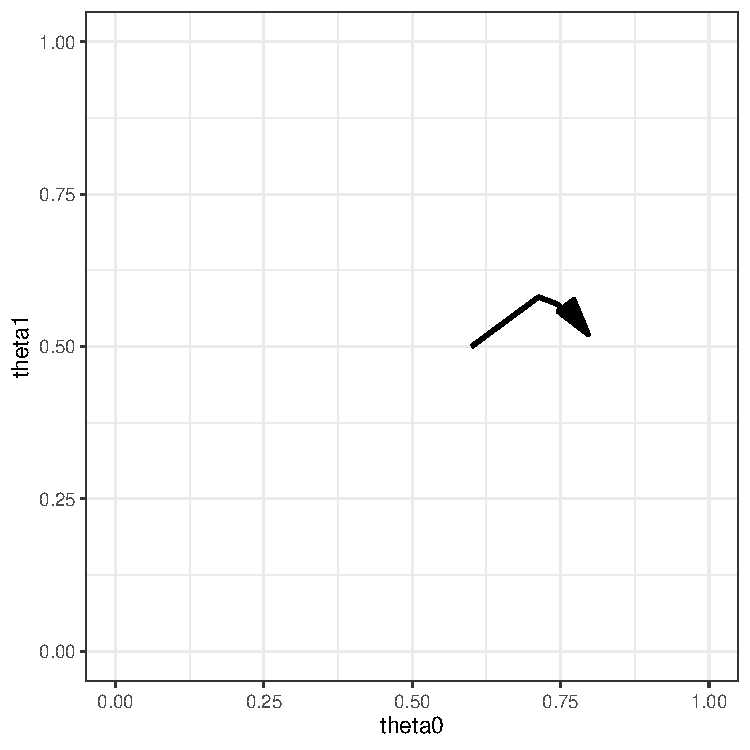
\includegraphics[page=1,keepaspectratio,width=\textwidth]{./source/em_figure1.pdf}
\end{center}
\normalsize
\end{column}
\end{columns}
\end{frame}


\begin{frame}[label={sec:org920b430}]{Multiple Initialization and Label Indeterminancy}
\begin{columns}
\begin{column}{0.50\columnwidth}
\begin{itemize}
\item Multiple initial starting parameters are often helpful.
\item In this instance, at least three \(\bthetahat\) seem to exist: (0.80, 0.52), (0.52, 0.80), (0.66, 0.66).
\item Note \(\btheta = (0.80, 0.52)\) and \(\btheta = (0.52, 0.80)\) give the same models because the labeling \(\theta_{0}\) and \(\theta_{1}\) (which coin we call 0 or 1) is arbitrary.
\item \(\btheta = (0.66, 0.66)\) corresponds to a model where we really only have one type of coins.
\end{itemize}
\end{column}

\begin{column}{0.50\columnwidth}
\scriptsize
\begin{center}
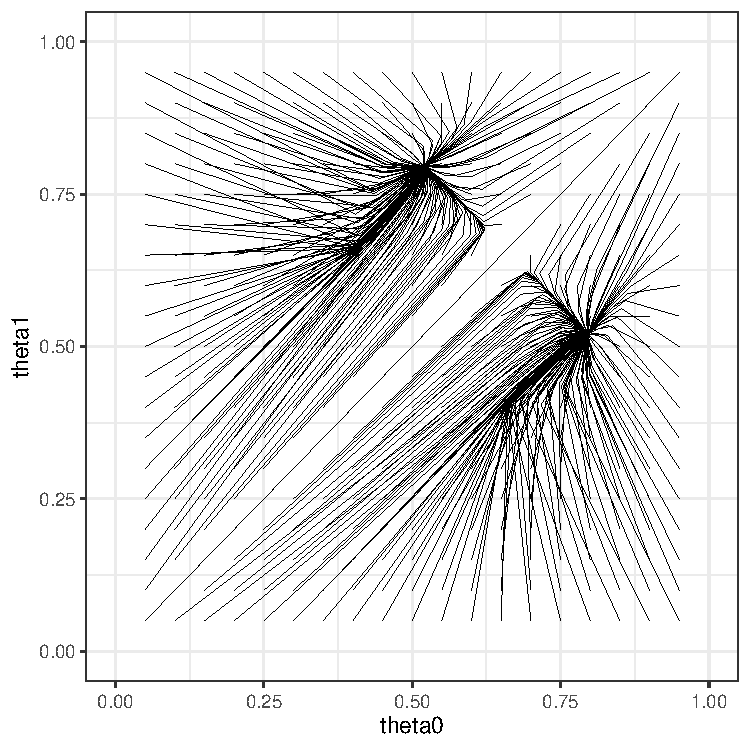
\includegraphics[page=1,keepaspectratio,width=\textwidth]{./source/em_figure2.pdf}
\end{center}
\normalsize
\end{column}
\end{columns}
\end{frame}

\begin{frame}[label={sec:orgae3a4fd}]{Incomplete-Data Likelihood}
\begin{columns}
\begin{column}{0.50\columnwidth}
\begin{itemize}
\item In this specific instance, the incomplete-data likelihood can be graphed with grid search as the parameter space is small and low dimensional ([0,1]\textsuperscript{2}).
\item The incomplete-data likelihood is bimodal and has a saddle point between the modes.
\item This shape explains the three solutions.
\end{itemize}
\end{column}

\begin{column}{0.50\columnwidth}
\scriptsize
\begin{center}
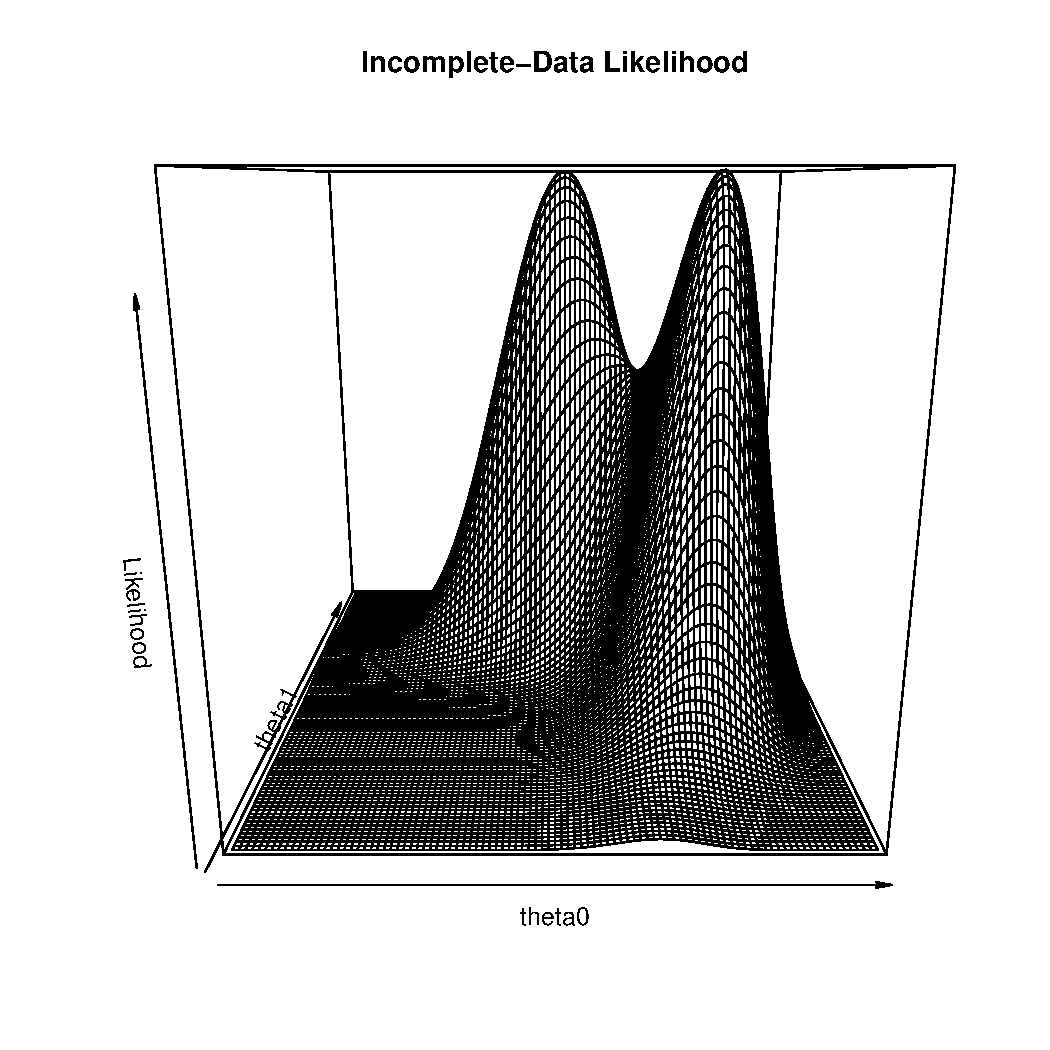
\includegraphics[width=.9\linewidth]{./source/likelihood2.pdf}
\end{center}
\end{column}
\end{columns}
\end{frame}

\begin{frame}[allowframebreaks,label=,t]{Incomplete-Data Likelihood Expression}
\begin{align*}
  &~~~\text{By iid}\\
  L(\btheta | \bx)
  &= \prod^{5}_{i=1}p(x_{i} | \btheta)\\
  &~~~\text{Introduce latent sate}\\
  &= \prod^{5}_{i=1} \sum^{1}_{z_{i}=0} p(x_{i}, z_{i} | \btheta)\\
  &= \prod^{5}_{i=1} \sum^{1}_{z_{i}=0} p(x_{i} | z_{i}, \btheta) p(z_{i} | \btheta)\\
  &~~~\text{$z_{i}$ does not depend on $\btheta$}\\
  &= \prod^{5}_{i=1} \sum^{1}_{z_{i}=0} p(x_{i} | z_{i}, \btheta) p(z_{i})\\
  &~~~\text{$p(z_{i})$ constant}\\
  &= \prod^{5}_{i=1} \sum^{1}_{z_{i}=0} p(x_{i} | z_{i}, \btheta) (0.5)\\
  &= \prod^{5}_{i=1} \sum^{1}_{z_{i}=0}
    (0.5) \binom{10}{x_{i}}
    \left[ \theta_{0}^{x_{i}}(1-\theta_{0})^{10-x_{i}} \right]^{1-z_{i}}
    \left[ \theta_{1}^{x_{i}}(1-\theta_{1})^{10-x_{i}} \right]^{z_{i}}\\
\end{align*}
\end{frame}


\begin{frame}[label={sec:orgd0aafc6}]{EM Algorithm Applications}
\begin{itemize}
\item Many probabilistic models in computational biology include latent variables. \cite{doWhatExpectationMaximization2008}
\begin{itemize}
\item Gene expression clustering
\item Motif finding
\item Haplotype inference
\end{itemize}
\end{itemize}
\end{frame}

\begin{frame}[allowframebreaks,label=,t]{Monotone Improvement in EM Algorithm}
\begin{itemize}
\item This part proves that the EM Algorithm is guaranteed to improve the parameter estimate toward the local optimum every step. \cite{doWhatExpectationMaximization2008,murphyMachineLearningProbabilistic2012}
\end{itemize}
\footnotesize
\begin{align*}
  \log \left( p(\bx | \btheta) \right)
  &= \log \left( \sum_{\bz} p(\bx, \bz | \btheta) \right)\\
  &~~~\text{Introduce arbitrary distribution $Q$}\\
  &= \log \left( \sum_{\bz} Q(\bz) \frac{p(\bx, \bz | \btheta)}{Q(\bz)} \right)\\
  &~~~\text{Rewrite as expectation}\\
  &= \log \left( E_{Q} \left[ \frac{p(\bx, \bz | \btheta)}{Q(\bz)} \right] \right)\\
  &~~~\text{Jensen's inequality on concave log}\\
  &\ge E_{Q} \left[ \log \left( \frac{p(\bx, \bz | \btheta)}{Q(\bz)} \right) \right]\\
  &= \sum_{\bz} Q(\bz) \log \left( \frac{p(\bx, \bz | \btheta)}{Q(\bz)} \right)\\
  &= \sum_{\bz} Q(\bz) \log \left( \frac{p(\bz | \bx, \btheta) p(\bx | \btheta)}{Q(\bz)} \right)\\
  &= \sum_{\bz} Q(\bz) \log \left( \frac{p(\bz | \bx, \btheta)}{Q(\bz)} \right) + \sum_{\bz} Q(\bz) \log \left( p(\bx | \btheta) \right)\\
  &= \sum_{\bz} Q(\bz) \log \left( \frac{p(\bz | \bx, \btheta)}{Q(\bz)} \right) + \log \left( p(\bx | \btheta) \right) \sum_{\bz} Q(\bz)\\
  &= \log \left( p(\bx | \btheta) \right) + \sum_{\bz} Q(\bz) \log \left( \frac{p(\bz | \bx, \btheta)}{Q(\bz)} \right)\\
  &= \log \left( p(\bx | \btheta) \right) - \Kbb\Lbb \left( Q(\bz) || p(\bz | \bx, \btheta) \right)
\end{align*}
\normalsize
\begin{itemize}
\item This inequality gives the lower bound for \(\log \left( p(\bx | \btheta) \right)\) for all \(\btheta\).
\item This lower bound is improved (maximized) by reducing the KL divergence \cite{murphyMachineLearningProbabilistic2012} by setting \(Q(\bz) = p(\bz | \bx, \btheta)\), which also gives equality.
\item As \(\btheta\) is the unknown quantity that we want to estimate, we can use \(Q(\bz) = p(\bz | \bx, \bthetahat^{(t)})\) as our best available option. In this case, equality holds at \(\log \left( p(\bx | \bthetahat^{(t)}) \right)\).
\item Consider the following function \(g_{t}(\btheta)\), which uses \(Q(\bz) = p(\bz | \bx, \bthetahat^{(t)})\). Note that only the numerator term within the log has a free parameter \(\btheta\). \cite{doWhatExpectationMaximization2008}
\end{itemize}
\footnotesize
\begin{align*}
  g_{t}(\btheta) &= \sum_{\bz} p \left( \bz | \bx, \bthetahat^{(t)} \right) \log \left( \frac{p(\bx,\bz | \btheta)}{p \left( \bz | \bx, \bthetahat^{(t)} \right)} \right)
\end{align*}
\normalsize
\begin{itemize}
\item Note that \(\log \left( p(\bx | \btheta) \right) \ge g_{t}(\btheta)\) for all \(\btheta\) by the inequality.
\item At \(\bthetahat^{(t)}\), \(g_{t}(\bthetahat^{(t)})\) meets the equality condition, thus, \(g_{t}(\bthetahat^{(t)}) = \log p(\bx | \bthetahat^{(t)})\). That is, \(g_{t}\) "touches" the incomplete-data likelihood function at the current parameter estimates. \cite{murphyMachineLearningProbabilistic2012}
\item Consider an update rule to find \(\btheta^{(t+1)}\) that maximizes this \(g_{t}\) function: \(\bthetahat^{(t+1)} = \arg\max_{\btheta} g_{t}(\btheta)\). Then the following inequality holds.
\end{itemize}
\footnotesize
\begin{align*}
  &~~~\text{By above inequality}\\
  \log p \left( \bx | \bthetahat^{(t+1)} \right)
  &\ge g_{t}\left( \bthetahat^{(t+1)} \right)\\
  &~~~\text{As $\bthetahat^{(t+1)}$ maximizes $g_{t}$}\\
  &\ge g_{t}\left( \bthetahat^{(t)} \right)\\
  &~~~\text{Equality holds at current value}\\
  &= \log p \left( \bx | \bthetahat^{(t)} \right)
\end{align*}
\normalsize
\begin{itemize}
\item Therefore, \(\log p \left( \bx | \bthetahat^{(t+1)} \right) \ge \log p \left( \bx | \bthetahat^{(t)} \right)\). That is, this update rule is guaranteed to improve the parameter estimate for the incomplete-data likelihood at each step.
\item Now compare this update rule to the EM algorithm.
\end{itemize}
\footnotesize
\begin{align*}
  \bthetahat^{(t+1)}
  &= \arg\max_{\btheta} g_{t}(\btheta)\\
  &= \arg\max_{\btheta} \sum_{\bz} p \left( \bz | \bx, \bthetahat^{(t)} \right) \log \left( \frac{p(\bx,\bz | \btheta)}{p \left( \bz | \bx, \bthetahat^{(t)} \right)} \right)\\
  &= \arg\max_{\btheta} \sum_{\bz} p \left( \bz | \bx, \bthetahat^{(t)} \right)
    \left[
    \log p(\bx,\bz | \btheta)
    -
    \log p \left( \bz | \bx, \bthetahat^{(t)} \right)
    \right]\\
  &~~~\text{Drop constant second term free of $\btheta$}\\
  &= \arg\max_{\btheta} \sum_{\bz} p \left( \bz | \bx, \bthetahat^{(t)} \right) \log p(\bx,\bz | \btheta)
\end{align*}
\normalsize
\begin{itemize}
\item This is maximization of the expected complete-data log likelihood. The expectation is over the distribution \(\bz\) given the observed data \(\bx\) and assuming the current parameter value \(\bthetahat^{(t)}\).
\item Therefore, the EM algorithm is equivalent to the update rule with the guaranteed improvement at each step.
\end{itemize}
\end{frame}

\begin{frame}[label={sec:orgc6f55ce}]{EM: Incomplete-Data Likelihood}
\begin{columns}
\begin{column}{0.50\columnwidth}
\begin{itemize}
\item Incomplete-data likelihood function.
\item \href{https://github.com/kaz-yos/em\_da\_repo/blob/master/source/em\_rgl.gif}{Animated gif on Github}
\end{itemize}
\end{column}

\begin{column}{0.50\columnwidth}
\begin{center}
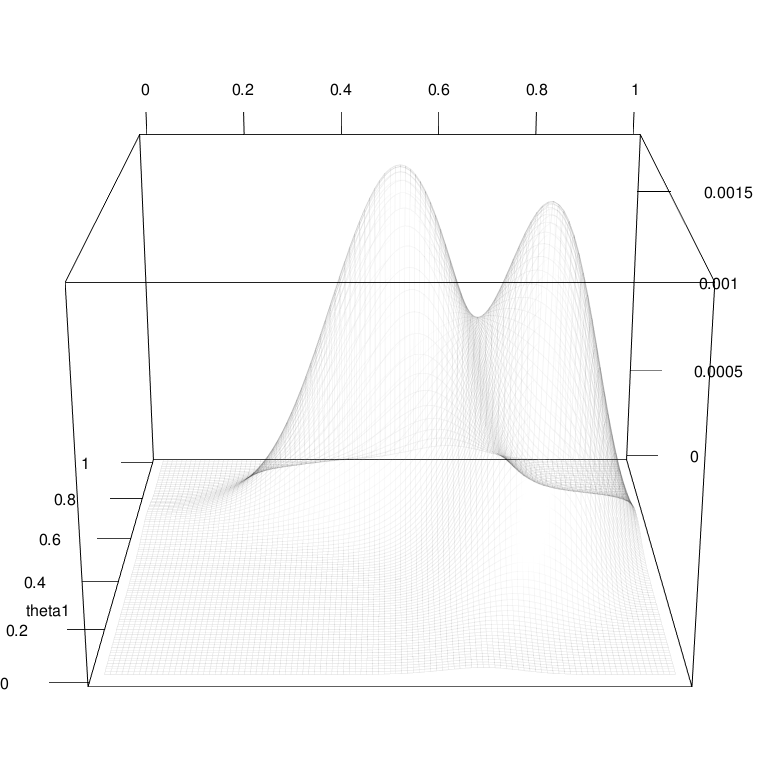
\includegraphics[page=1,keepaspectratio,width=\textwidth,height=\textheight]{./source/em_rgl_.png}
\end{center}
\end{column}
\end{columns}
\end{frame}

\begin{frame}[label={sec:org254062f}]{EM: E Step (0)}
\begin{columns}
\begin{column}{0.50\columnwidth}
\begin{itemize}
\item \(g_{0}(\theta)\) added
\end{itemize}
\end{column}
\begin{column}{0.50\columnwidth}
\begin{center}
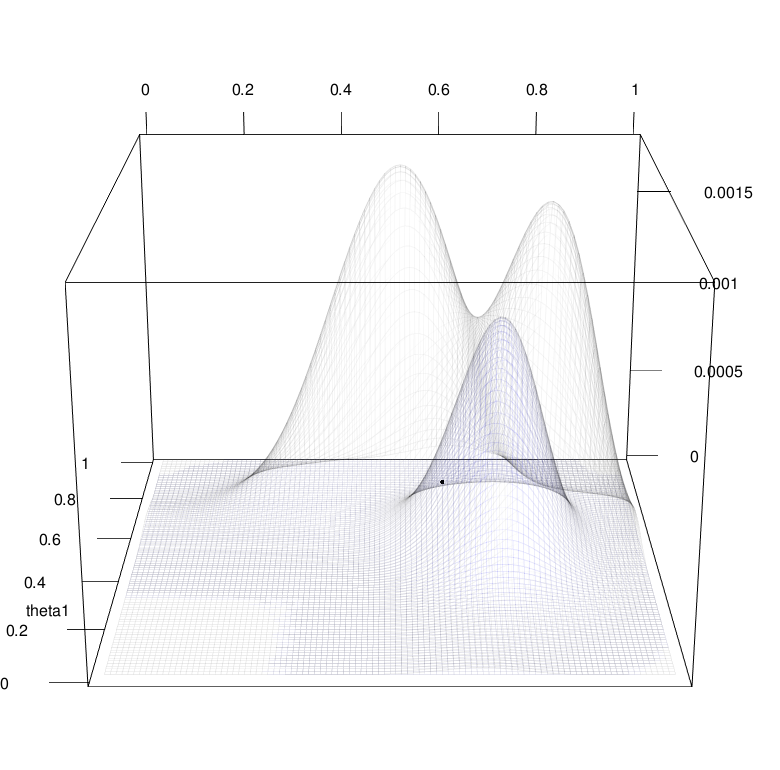
\includegraphics[page=1,keepaspectratio,width=\textwidth,height=\textheight]{./source/em_rgl_g0_e.png}
\end{center}
\end{column}
\end{columns}
\end{frame}

\begin{frame}[label={sec:org925f2ee}]{EM: M Step (0)}
\begin{columns}
\begin{column}{0.50\columnwidth}
\begin{itemize}
\item \(g_{0}(\theta)\) maximized
\end{itemize}
\end{column}
\begin{column}{0.50\columnwidth}
\begin{center}
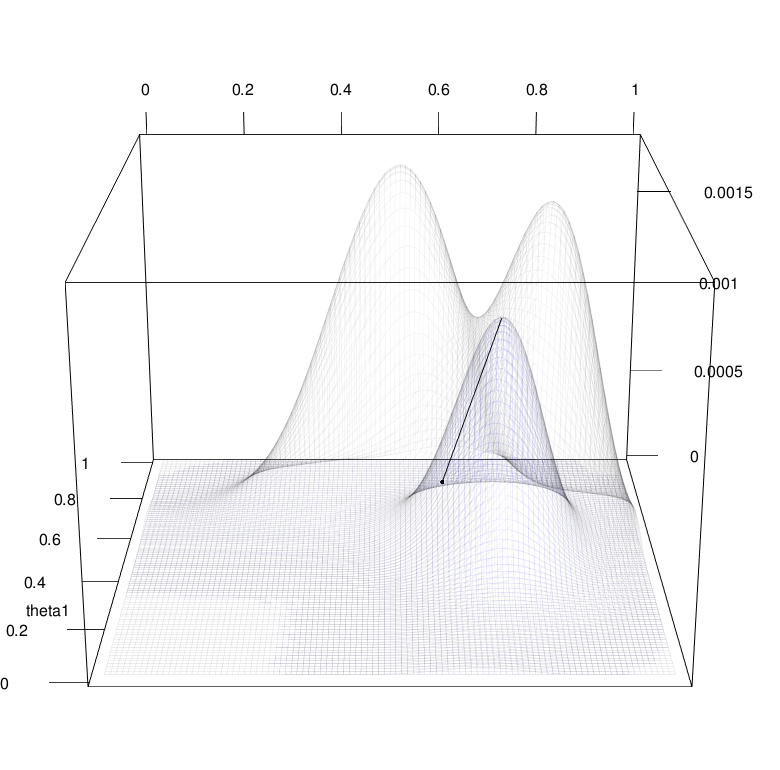
\includegraphics[page=1,keepaspectratio,width=\textwidth,height=\textheight]{./source/em_rgl_g0_m.png}
\end{center}
\end{column}
\end{columns}
\end{frame}

\begin{frame}[label={sec:org3a727d7}]{EM: E Step (1)}
\begin{columns}
\begin{column}{0.50\columnwidth}
\begin{itemize}
\item \(g_{1}(\theta)\) added
\end{itemize}
\end{column}
\begin{column}{0.50\columnwidth}
\begin{center}
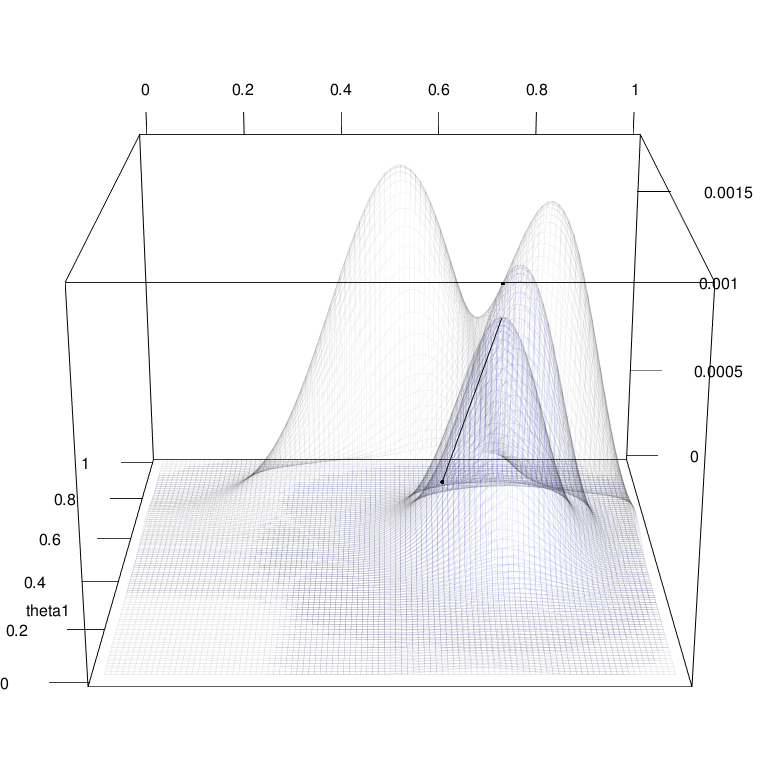
\includegraphics[page=1,keepaspectratio,width=\textwidth,height=\textheight]{./source/em_rgl_g1_e.png}
\end{center}
\end{column}
\end{columns}
\end{frame}

\begin{frame}[label={sec:orgee1b867}]{EM: M Step (1)}
\begin{columns}
\begin{column}{0.50\columnwidth}
\begin{itemize}
\item \(g_{1}(\theta)\) maximized
\end{itemize}
\end{column}
\begin{column}{0.50\columnwidth}
\begin{center}
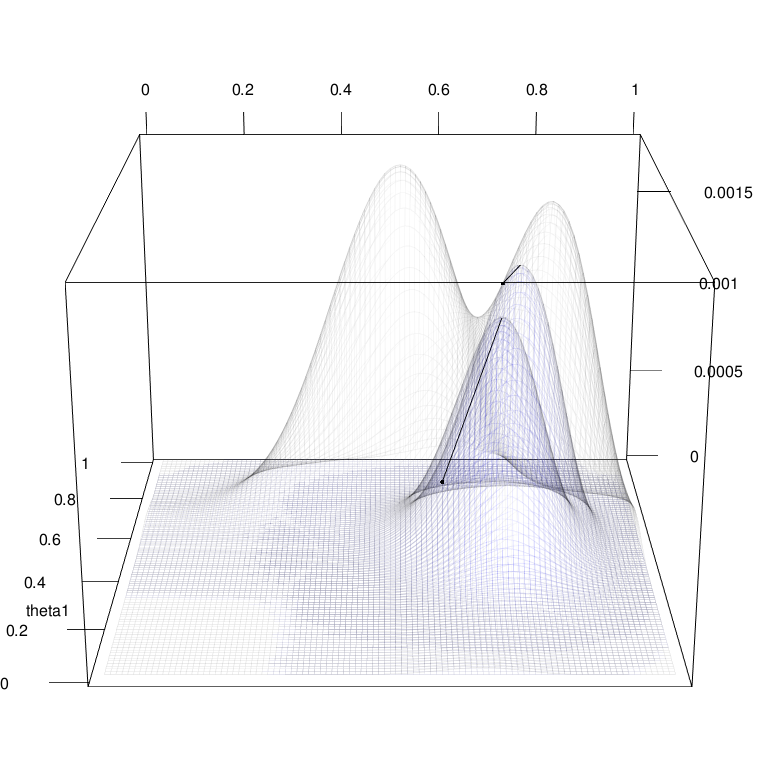
\includegraphics[page=1,keepaspectratio,width=\textwidth,height=\textheight]{./source/em_rgl_g1_m.png}
\end{center}
\end{column}
\end{columns}
\end{frame}

\begin{frame}[label={sec:org3c3d536}]{EM: E Step (2)}
\begin{columns}
\begin{column}{0.50\columnwidth}
\begin{itemize}
\item \(g_{2}(\theta)\) added
\end{itemize}
\end{column}
\begin{column}{0.50\columnwidth}
\begin{center}
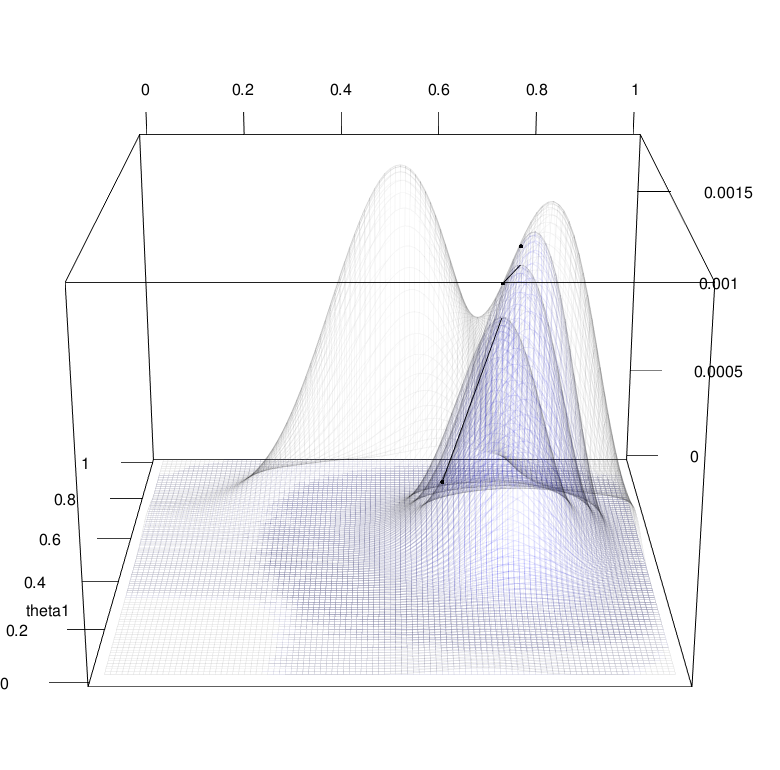
\includegraphics[page=1,keepaspectratio,width=\textwidth,height=\textheight]{./source/em_rgl_g2_e.png}
\end{center}
\end{column}
\end{columns}
\end{frame}

\begin{frame}[label={sec:org5a5a9ef}]{EM: M Step (2)}
\begin{columns}
\begin{column}{0.50\columnwidth}
\begin{itemize}
\item \(g_{2}(\theta)\) maximized
\end{itemize}
\end{column}
\begin{column}{0.50\columnwidth}
\begin{center}
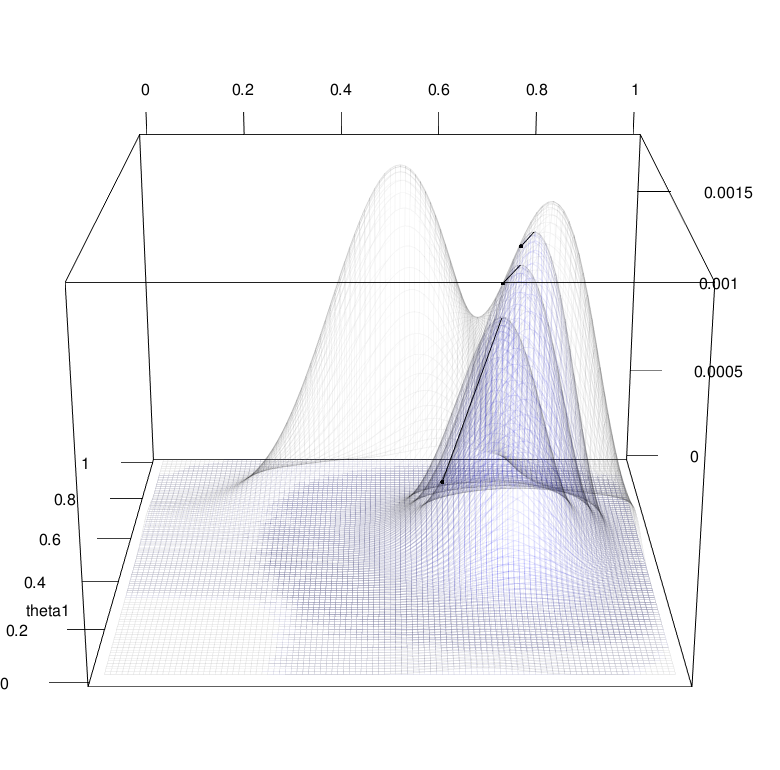
\includegraphics[page=1,keepaspectratio,width=\textwidth,height=\textheight]{./source/em_rgl_g2_m.png}
\end{center}
\end{column}
\end{columns}
\end{frame}

\begin{frame}[label={sec:orga1e03c9}]{EM: E Step (3)}
\begin{columns}
\begin{column}{0.50\columnwidth}
\begin{itemize}
\item \(g_{3}(\theta)\) added
\end{itemize}
\end{column}
\begin{column}{0.50\columnwidth}
\begin{center}
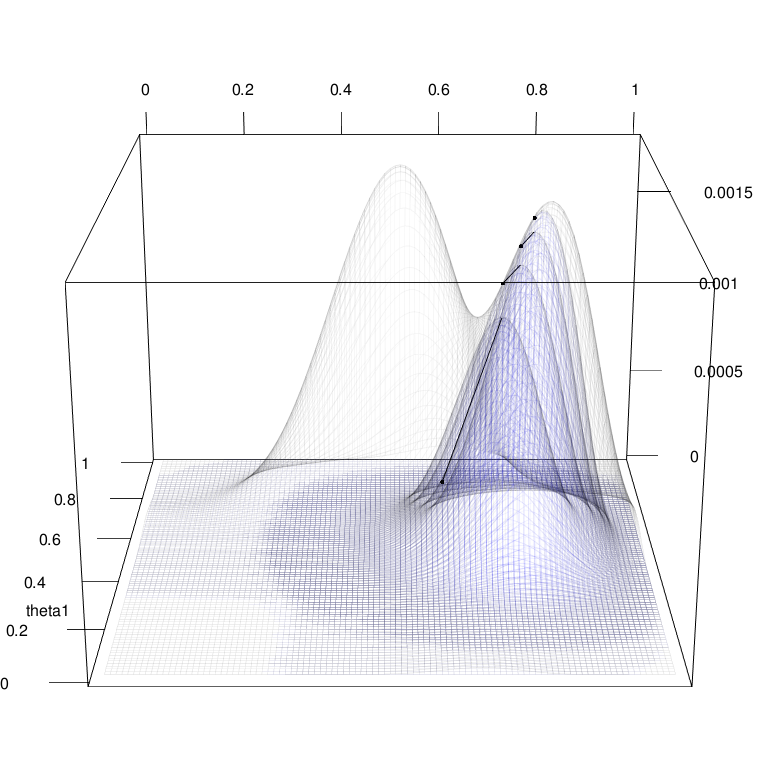
\includegraphics[page=1,keepaspectratio,width=\textwidth,height=\textheight]{./source/em_rgl_g3_e.png}
\end{center}
\end{column}
\end{columns}
\end{frame}

\begin{frame}[label={sec:orgbae1487}]{EM: M Step (3)}
\begin{columns}
\begin{column}{0.50\columnwidth}
\begin{itemize}
\item \(g_{3}(\theta)\) maximized
\end{itemize}
\end{column}
\begin{column}{0.50\columnwidth}
\begin{center}
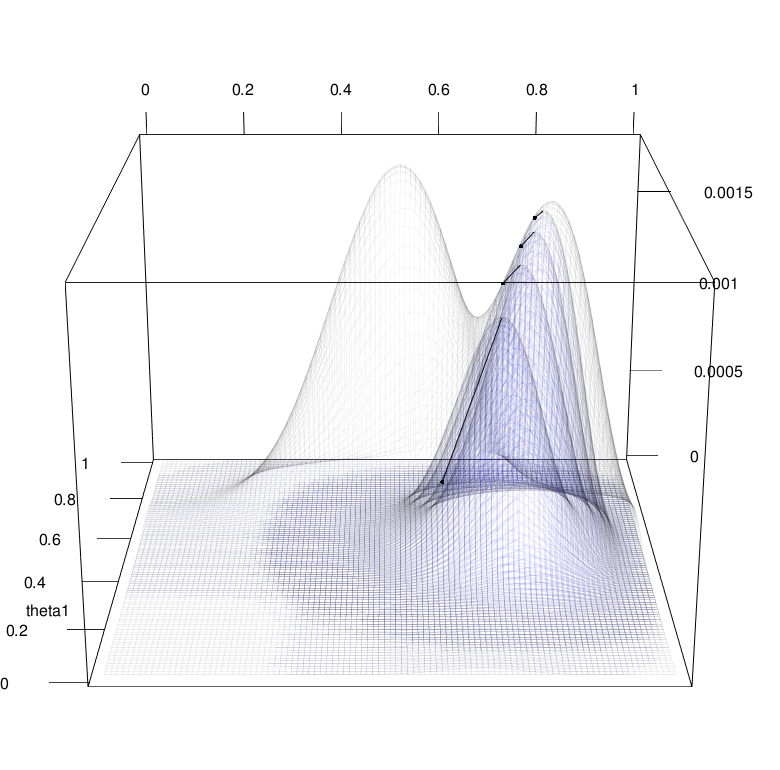
\includegraphics[page=1,keepaspectratio,width=\textwidth,height=\textheight]{./source/em_rgl_g3_m.png}
\end{center}
\end{column}
\end{columns}
\end{frame}

\begin{frame}[label={sec:orga874369}]{EM: E Step (4)}
\begin{columns}
\begin{column}{0.50\columnwidth}
\begin{itemize}
\item \(g_{4}(\theta)\) added
\end{itemize}
\end{column}
\begin{column}{0.50\columnwidth}
\begin{center}
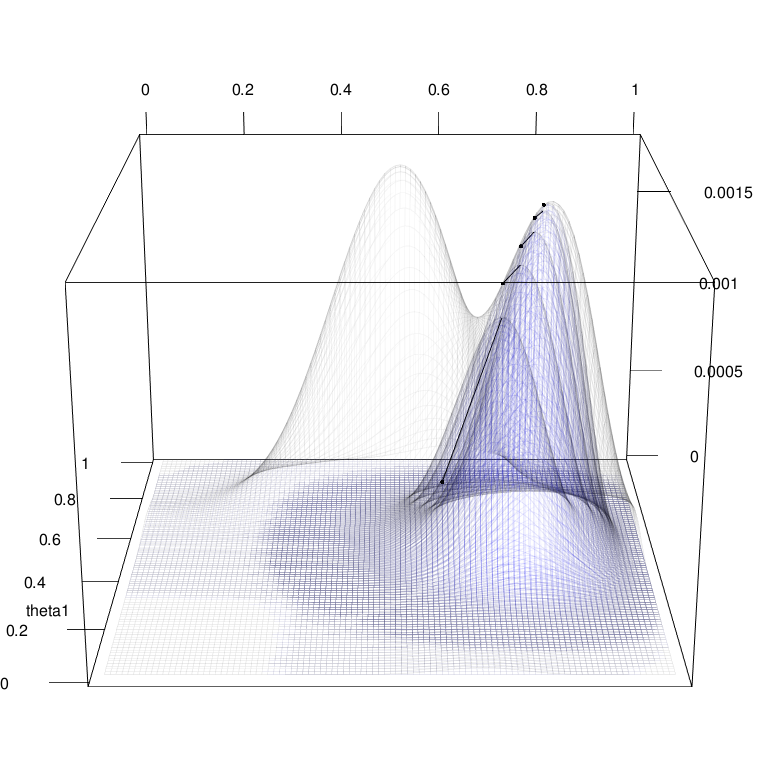
\includegraphics[page=1,keepaspectratio,width=\textwidth,height=\textheight]{./source/em_rgl_g4_e.png}
\end{center}
\end{column}
\end{columns}
\end{frame}

\begin{frame}[label={sec:orgf00e319}]{EM: M Step (4)}
\begin{columns}
\begin{column}{0.50\columnwidth}
\begin{itemize}
\item \(g_{4}(\theta)\) maximized
\end{itemize}
\end{column}
\begin{column}{0.50\columnwidth}
\begin{center}
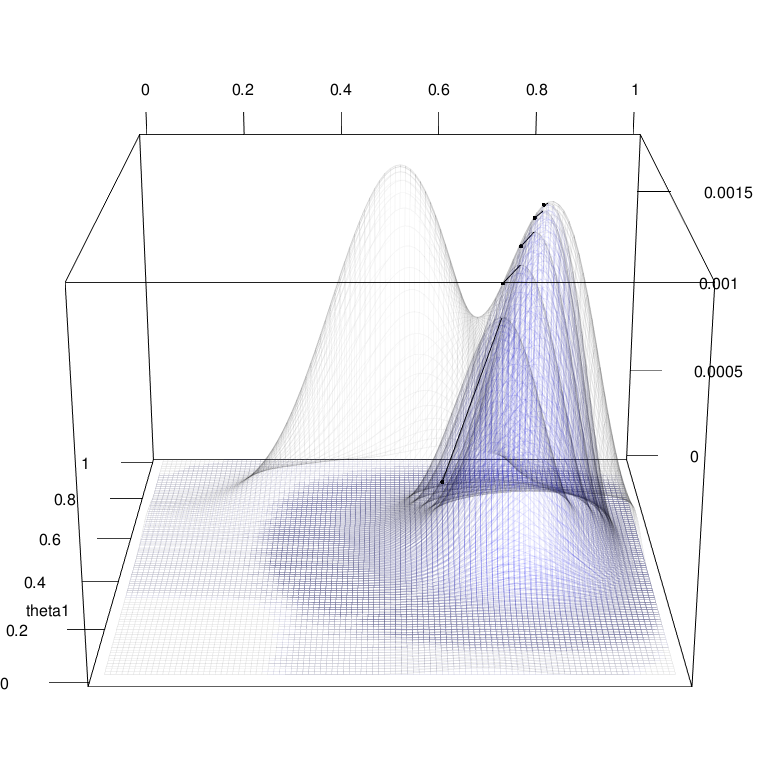
\includegraphics[page=1,keepaspectratio,width=\textwidth,height=\textheight]{./source/em_rgl_g4_m.png}
\end{center}
\end{column}
\end{columns}
\end{frame}

\begin{frame}[label={sec:org941a524}]{EM: E Step (5)}
\begin{columns}
\begin{column}{0.50\columnwidth}
\begin{itemize}
\item \(g_{5}(\theta)\) added
\end{itemize}
\end{column}
\begin{column}{0.50\columnwidth}
\begin{center}
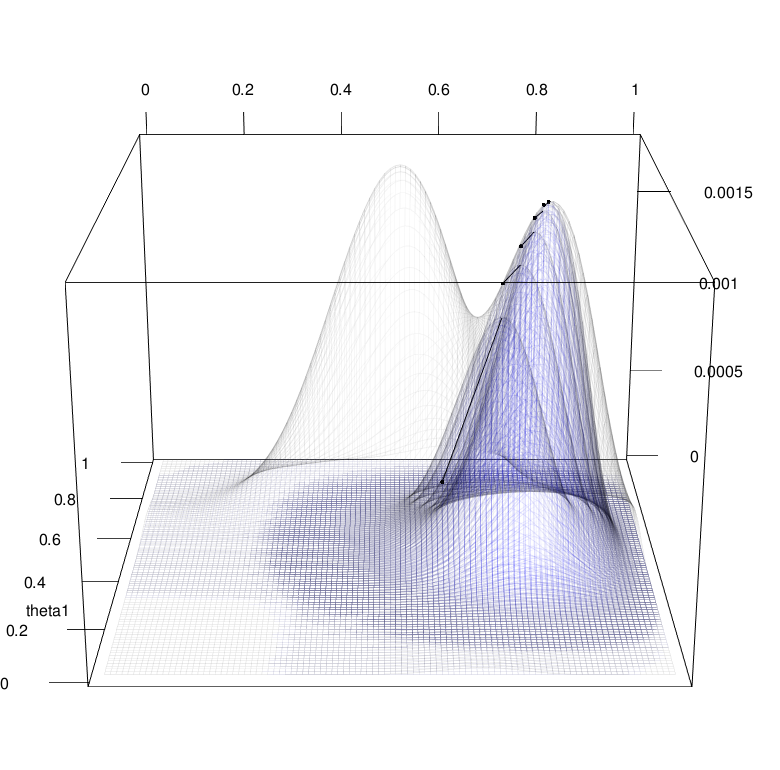
\includegraphics[page=1,keepaspectratio,width=\textwidth,height=\textheight]{./source/em_rgl_g5_e.png}
\end{center}
\end{column}
\end{columns}
\end{frame}

\begin{frame}[label={sec:orgc761e16}]{EM: M Step (5)}
\begin{columns}
\begin{column}{0.50\columnwidth}
\begin{itemize}
\item \(g_{5}(\theta)\) maximized
\end{itemize}
\end{column}
\begin{column}{0.50\columnwidth}
\begin{center}
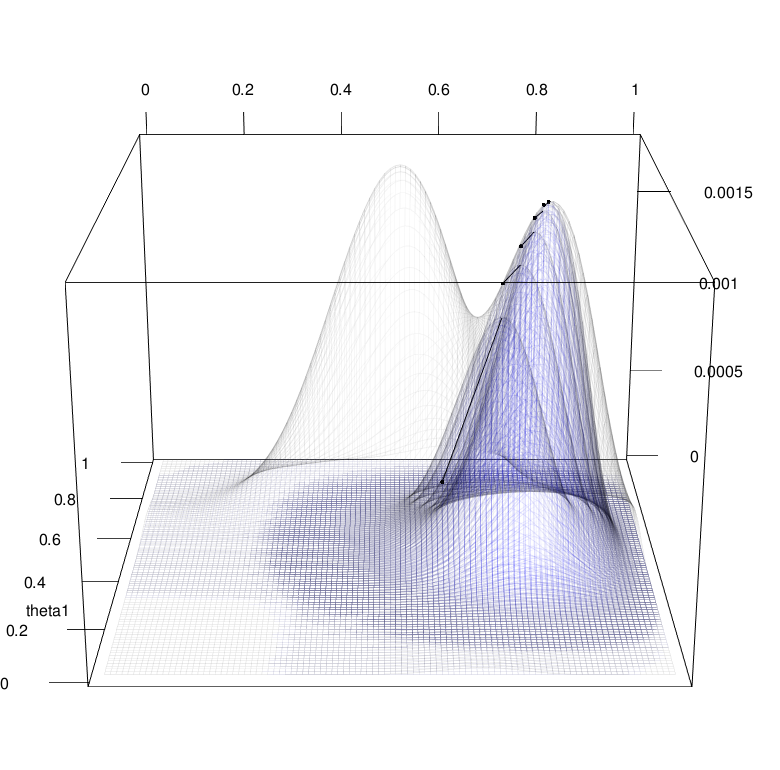
\includegraphics[page=1,keepaspectratio,width=\textwidth,height=\textheight]{./source/em_rgl_g5_m.png}
\end{center}
\end{column}
\end{columns}
\end{frame}

\section{DA Method}
\label{sec:org536f30f}
\appendix
\begin{frame}[label={sec:org48f9767}]{}
\begin{center}
\resizebox{\linewidth}{!}{Data Augmentation Method}
\end{center}
\end{frame}

\begin{frame}[label={sec:org304459e}]{From EM to DA}
\begin{itemize}
\item A related Bayesian computation method is the \emph{Data Augmentation} method. \cite{tannerCalculationPosteriorDistributions1987,tannerEMDataAugmentation2010}
\item Here we treat the simplest case that reduces to the two-step Gibbs sampling. \cite{gemanStochasticRelaxationGibbs1984,vandykArtDataAugmentation2001}
\item After random initialization of parameters, two steps alternates until convergence to a posterior distribution.
\begin{enumerate}
\item Imputation (I) Step:
\begin{itemize}
\item Estimate probabilities of latent states given current parameters
\item Draw a latent state
\end{itemize}
\item Posterior (P) Step:
\begin{itemize}
\item Draw new parameters given data and latent state
\end{itemize}
\end{enumerate}
\item The resulting parameter draws from the later sequence approximate draws from the target posterior.
\end{itemize}
\end{frame}

\begin{frame}[label={sec:org8911973}]{Model Configuration}
\begin{itemize}
\item To set up a Bayesian computation, we need probability models for the data (likelihood) as well as the parameters (prior).
\item Likelihood
\end{itemize}
\begin{align*}
  Z_{i} &\sim \text{Bernoulli}(p = 0.5), Z_{i} \in \left\{ 0,1 \right\}\\
  X_{i} | Z_{i}, \btheta &\sim \text{Binomial}(n = 10, p = \theta_{Z_{i}}), X_{i} \in \left\{ 0, \dots, 10 \right\}
\end{align*}
\begin{itemize}
\item Prior
\end{itemize}
\begin{align*}
  \theta_{0} &\sim \text{Beta}(a_{0},b_{0})\\
  \theta_{1} &\sim \text{Beta}(a_{1},b_{1})
\end{align*}
\begin{itemize}
\item Here we will consider independent uniform priors (\(a_{j} = b_{j} = 1, j = 0,1\)).
\end{itemize}
\end{frame}

\begin{frame}[label={sec:org37b87fc}]{Parameter Initialization}
\begin{itemize}
\item Randomly initialize the parameters
\begin{itemize}
\item \(\theta_{0}^{(0)} := 0.6\)
\item \(\theta_{1}^{(0)} := 0.5\)
\end{itemize}
\end{itemize}
\end{frame}

\begin{frame}[fragile,allowframebreaks,label=,t]{I-Step (1)}
 \begin{itemize}
\item Current parameters: \(\theta_{0}^{(0)} = 0.6, \theta_{1}^{(0)} = 0.5\)
\end{itemize}
\footnotesize
\begin{center}
\begin{tabular}{r|l|ll|r|ll|}
Index & Coin & Prob. Coin A & Prob. Coin B & Heads & Heads Coin A & Heads Coin B\\
\(i\) & \(Z_{i}\) & \(E[(1-Z_{i})\vert X_{i}]\) & \(E[Z_{i}\vert X_{i}]\) & \(X_{i}\) & \(E[(1-Z_{i}) X_{i} \vert X_{i}]\) & \(E[Z_{i} X_{i} \vert X_{i}]\)\\
\hline
1 & ? & ? & ? & 5 & ? \texttimes{} 5 & ? \texttimes{} 5\\
2 & ? & ? & ? & 9 & ? \texttimes{} 9 & ? \texttimes{} 9\\
3 & ? & ? & ? & 8 & ? \texttimes{} 8 & ? \texttimes{} 8\\
4 & ? & ? & ? & 4 & ? \texttimes{} 4 & ? \texttimes{} 4\\
5 & ? & ? & ? & 7 & ? \texttimes{} 7 & ? \texttimes{} 7\\
\hline
Sum &  &  &  & 33 & ? & ?\\
\end{tabular}
\end{center}
\normalsize
\begin{itemize}
\item First, we need coin probabilities for each \(i\) given the current parameter values \(\btheta^{(0)}\).
\item This calculation is the same as the EM algorithm.
\end{itemize}

\newpage
\begin{itemize}
\item Now we have the probabilities of coin identities.
\end{itemize}
\footnotesize
\begin{center}
\begin{tabular}{r|l|rr|r|ll|}
Index & Coin & Prob. Coin A & Prob. Coin B & Heads & Heads Coin A & Heads Coin B\\
\(i\) & \(Z_{i}\) & \(E[(1-Z_{i})\vert X_{i}]\) & \(E[Z_{i}\vert X_{i}]\) & \(X_{i}\) & \(E[(1-Z_{i}) X_{i} \vert X_{i}]\) & \(E[Z_{i} X_{i} \vert X_{i}]\)\\
\hline
1 & ? & 0.45 & 0.55 & 5 & ? \texttimes{} 5 & ? \texttimes{} 5\\
2 & ? & 0.80 & 0.20 & 9 & ? \texttimes{} 9 & ? \texttimes{} 9\\
3 & ? & 0.73 & 0.27 & 8 & ? \texttimes{} 8 & ? \texttimes{} 8\\
4 & ? & 0.35 & 0.65 & 4 & ? \texttimes{} 4 & ? \texttimes{} 4\\
5 & ? & 0.65 & 0.35 & 7 & ? \texttimes{} 7 & ? \texttimes{} 7\\
\hline
Sum &  &  &  & 33 & ? & ?\\
\end{tabular}
\end{center}
\normalsize
\begin{itemize}
\item We will now draw \(Z_{i}^{(1)}\).
\end{itemize}
\scriptsize
\begin{minted}[frame=lines,linenos=false]{r}
set.seed(737265171)
rbinom(n = 5, size = 1, prob = c(0.55, 0.20, 0.27, 0.65, 0.35))
\end{minted}

\begin{verbatim}

[1] 0 0 0 1 0
\end{verbatim}


\normalsize

\newpage
\begin{itemize}
\item We have imputed the latent coin identities.
\end{itemize}
\footnotesize
\begin{center}
\begin{tabular}{r|r|rr|r|ll|}
Index & Coin & Prob. Coin A & Prob. Coin B & Heads & Heads Coin A & Heads Coin B\\
\(i\) & \(Z_{i}\) & \(E[(1-Z_{i})\vert X_{i}]\) & \(E[Z_{i}\vert X_{i}]\) & \(X_{i}\) & \(E[(1-Z_{i}) X_{i} \vert X_{i}]\) & \(E[Z_{i} X_{i} \vert X_{i}]\)\\
\hline
1 & 0 & 0.45 & 0.55 & 5 & ? \texttimes{} 5 & ? \texttimes{} 5\\
2 & 0 & 0.80 & 0.20 & 9 & ? \texttimes{} 9 & ? \texttimes{} 9\\
3 & 0 & 0.73 & 0.27 & 8 & ? \texttimes{} 8 & ? \texttimes{} 8\\
4 & 1 & 0.35 & 0.65 & 4 & ? \texttimes{} 4 & ? \texttimes{} 4\\
5 & 0 & 0.65 & 0.35 & 7 & ? \texttimes{} 7 & ? \texttimes{} 7\\
\hline
Sum &  &  &  & 33 & ? & ?\\
\end{tabular}
\end{center}
\normalsize
\begin{itemize}
\item We will proceed assuming these imputed latent coin identities.
\end{itemize}

\newpage
\begin{itemize}
\item We have imputed the latent coin identities.
\end{itemize}
\footnotesize
\begin{center}
\begin{tabular}{r|r|rr|r|ll|}
Index & Coin & Prob. Coin A & Prob. Coin B & Heads & Heads Coin A & Heads Coin B\\
\(i\) & \(Z_{i}\) & \(E[(1-Z_{i})\vert X_{i}]\) & \(E[Z_{i}\vert X_{i}]\) & \(X_{i}\) & \(E[(1-Z_{i}) X_{i} \vert X_{i}]\) & \(E[Z_{i} X_{i} \vert X_{i}]\)\\
\hline
1 & 0 & 0.45 & 0.55 & 5 & 1 \texttimes{} 5 & 0 \texttimes{} 5\\
2 & 0 & 0.80 & 0.20 & 9 & 1 \texttimes{} 9 & 0 \texttimes{} 9\\
3 & 0 & 0.73 & 0.27 & 8 & 1 \texttimes{} 8 & 0 \texttimes{} 8\\
4 & 1 & 0.35 & 0.65 & 4 & 0 \texttimes{} 4 & 1 \texttimes{} 4\\
5 & 0 & 0.65 & 0.35 & 7 & 1 \texttimes{} 7 & 0 \texttimes{} 7\\
\hline
Sum &  &  &  & 33 & 29 & 4\\
\end{tabular}
\end{center}
\normalsize
\begin{itemize}
\item We will proceed assuming these imputed latent coin identities.
\end{itemize}
\end{frame}


\begin{frame}[fragile,allowframebreaks,label=,t]{P-Step (1)}
 \begin{itemize}
\item Now using the complete data on \((\bZ,\bX)\), construct a posterior \(p(\btheta | \bZ, \bX)\).
\end{itemize}
\footnotesize
\begin{center}
\begin{tabular}{r|r|rr|r|ll|}
Index & Coin & Prob. Coin A & Prob. Coin B & Heads & Heads Coin A & Heads Coin B\\
\(i\) & \(Z_{i}\) & \(E[(1-Z_{i})\vert X_{i}]\) & \(E[Z_{i}\vert X_{i}]\) & \(X_{i}\) & \(E[(1-Z_{i}) X_{i} \vert X_{i}]\) & \(E[Z_{i} X_{i} \vert X_{i}]\)\\
\hline
1 & 0 & 0.45 & 0.55 & 5 & 1 \texttimes{} 5 & 0 \texttimes{} 5\\
2 & 0 & 0.80 & 0.20 & 9 & 1 \texttimes{} 9 & 0 \texttimes{} 9\\
3 & 0 & 0.73 & 0.27 & 8 & 1 \texttimes{} 8 & 0 \texttimes{} 8\\
4 & 1 & 0.35 & 0.65 & 4 & 0 \texttimes{} 4 & 1 \texttimes{} 4\\
5 & 0 & 0.65 & 0.35 & 7 & 1 \texttimes{} 7 & 0 \texttimes{} 7\\
\hline
Sum &  &  &  &  & 29 & 4\\
\end{tabular}
\end{center}
\normalsize
\begin{itemize}
\item Using imputed coin identities, we have 29 head and 11 tails (40 tosses) for Coin A and 4 heads and 6 tails (10 tosses) for Coin B.
\end{itemize}

\newpage
\begin{itemize}
\item By conjugacy, we can updated the beta distributions as follows.
\end{itemize}
\begin{align*}
  \theta_{0}^{(1)} &\sim \text{Beta}(1 + 29, 1 + 11)\\
  \theta_{1}^{(1)} &\sim \text{Beta}(1 + 4, 1 + 6)
\end{align*}
\begin{itemize}
\item Draw updated values.
\end{itemize}
\tiny
\begin{minted}[frame=lines,linenos=false]{r}
c(rbeta(n = 1, shape1 = 1 + 29, shape2 = 1 + 11),
  rbeta(n = 1, shape1 = 1 +  4, shape2 = 1 +  6)) %>% round(3)
\end{minted}

\begin{verbatim}

[1] 0.760 0.471
\end{verbatim}


\normalsize
\begin{itemize}
\item We now have updated parameter draws: \(\thetahat_{0}^{(1)} := 0.760\); \(\thetahat_{1}^{(1)} := 0.471\)
\end{itemize}
\end{frame}

\begin{frame}[fragile,allowframebreaks,label=,t]{I-Step (2)}
 \begin{itemize}
\item Current parameters: \(\theta_{0}^{(1)} = 0.760, \theta_{1}^{(1)} = 0.471\)
\item Calculate the probabilities again and impute the latent states.
\end{itemize}
\footnotesize
\begin{center}
\begin{tabular}{r|r|rr|r|ll|}
Index & Coin & Prob. Coin A & Prob. Coin B & Heads & Heads Coin A & Heads Coin B\\
\(i\) & \(Z_{i}\) & \(E[(1-Z_{i})\vert X_{i}]\) & \(E[Z_{i}\vert X_{i}]\) & \(X_{i}\) & \(E[(1-Z_{i}) X_{i} \vert X_{i}]\) & \(E[Z_{i} X_{i} \vert X_{i}]\)\\
\hline
1 & 1 & 0.17 & 0.83 & 5 & 0 \texttimes{} 5 & 1 \texttimes{} 5\\
2 & 0 & 0.97 & 0.03 & 9 & 1 \texttimes{} 9 & 0 \texttimes{} 9\\
3 & 0 & 0.90 & 0.10 & 8 & 1 \texttimes{} 8 & 0 \texttimes{} 8\\
4 & 1 & 0.06 & 0.94 & 4 & 0 \texttimes{} 4 & 1 \texttimes{} 4\\
5 & 0 & 0.73 & 0.27 & 7 & 1 \texttimes{} 7 & 0 \texttimes{} 7\\
\hline
Sum &  &  &  & 33 & 24 & 9\\
\end{tabular}
\end{center}
\normalsize
\scriptsize
\begin{minted}[frame=lines,linenos=false]{r}
rbinom(n = 5, size = 1, prob = c(0.83, 0.03, 0.10, 0.94, 0.27))
\end{minted}

\begin{verbatim}
[1] 1 0 0 1 0
\end{verbatim}


\normalsize
\newpage
\begin{itemize}
\item Using imputed coin identities, we have 24 head and 6 tails (30 tosses) for Coin A and 9 heads and 11 tail (20 tosses) for Coin B.
\end{itemize}
\footnotesize
\begin{center}
\begin{tabular}{r|r|rr|r|ll|}
Index & Coin & Prob. Coin A & Prob. Coin B & Heads & Heads Coin A & Heads Coin B\\
\(i\) & \(Z_{i}\) & \(E[(1-Z_{i})\vert X_{i}]\) & \(E[Z_{i}\vert X_{i}]\) & \(X_{i}\) & \(E[(1-Z_{i}) X_{i} \vert X_{i}]\) & \(E[Z_{i} X_{i} \vert X_{i}]\)\\
\hline
1 & 1 & 0.17 & 0.83 & 5 & 0 \texttimes{} 5 & 1 \texttimes{} 5\\
2 & 0 & 0.97 & 0.03 & 9 & 1 \texttimes{} 9 & 0 \texttimes{} 9\\
3 & 0 & 0.90 & 0.10 & 8 & 1 \texttimes{} 8 & 0 \texttimes{} 8\\
4 & 1 & 0.06 & 0.94 & 4 & 0 \texttimes{} 4 & 1 \texttimes{} 4\\
5 & 0 & 0.73 & 0.27 & 7 & 1 \texttimes{} 7 & 0 \texttimes{} 7\\
\hline
Sum &  &  &  & 33 & 24 & 9\\
\end{tabular}
\end{center}
\normalsize
\end{frame}

\begin{frame}[fragile,allowframebreaks,label=,t]{P-Step (2)}
 \begin{itemize}
\item We have 24 head and 6 tails (30 tosses) for Coin A and 9 heads and 11 tail (20 tosses) for Coin B.
\item The posterior distributions are:
\end{itemize}
\begin{align*}
  \theta_{0}^{(2)} &\sim \text{Beta}(1 + 24, 1 + 6)\\
  \theta_{1}^{(2)} &\sim \text{Beta}(1 + 9, 1 + 11)
\end{align*}
\begin{itemize}
\item Draw updated values.
\end{itemize}
\scriptsize
\begin{minted}[frame=lines,linenos=false]{r}
c(rbeta(n = 1, shape1 = 1 + 24, shape2 = 1 +  6),
  rbeta(n = 1, shape1 = 1 +  9, shape2 = 1 + 11)) %>% round(3)
\end{minted}

\begin{verbatim}

[1] 0.677 0.483
\end{verbatim}


\normalsize
\begin{itemize}
\item We now have updated parameter draws.
\begin{itemize}
\item \(\theta_{0}^{(2)} := 0.677\)
\item \(\theta_{1}^{(2)} := 0.483\)
\end{itemize}
\end{itemize}


\begin{itemize}
\item In the limit, the draws for the missing data (I-Step) and the parameters (P-Step) are from the joint posterior \emph{distribution} of the missing data and the parameters. \cite{littleStatisticalAnalysisMissing2002}
\item Note that this algorithm does not converge to a point unlike the EM algorithm.
\end{itemize}
\end{frame}

\begin{frame}[fragile,allowframebreaks,label=,t]{Automated Version}
 \scriptsize
\begin{minted}[frame=lines,linenos=false]{r}
ip_step <- function(theta, a, b) {
  X <- c(5,9,8,4,7)
  imp_coin <- bind_rows(rel_dbinom(X[1], theta),
                        rel_dbinom(X[2], theta),
                        rel_dbinom(X[3], theta),
                        rel_dbinom(X[4], theta),
                        rel_dbinom(X[5], theta)) %>%
    mutate(Coin = rbinom(n = 5, size = 1,
                         prob = `Prob. Coin B`),
           X = X,
           `Heads Coin A` = X * (1 - Coin),
           `Heads Coin B` = X * Coin) %>%
    select(Coin, `Prob. Coin A`, `Prob. Coin B`,
           X, `Heads Coin A`, `Heads Coin B`)
  imp_coin <- bind_cols(tibble(Index = c(as.character(1:5), "Sum")),
                        bind_rows(imp_coin, colSums(imp_coin)))

  Heads_A <- imp_coin$`Heads Coin A`[6]
  Tails_A <- (5 - imp_coin$Coin[6]) * 10 - Heads_A
  Heads_B <- imp_coin$`Heads Coin B`[6]
  Tails_B <- imp_coin$Coin[6] * 10 - Heads_B
  theta_post_draws <- c(rbeta(n = 1, shape1 = a[1] + Heads_A, shape2 = b[1] + Tails_A),
                        rbeta(n = 1, shape1 = a[1] + Heads_B, shape2 = b[2] + Tails_B))

  list(I = imp_coin, P = theta_post_draws)
}

ip_iter <- function(theta, a = c(1,1), b = c(1,1), iter = 10) {
  thetas <- data.frame(theta0 = c(theta[1], rep(as.numeric(NA), iter)),
                       theta1 = c(theta[2], rep(as.numeric(NA), iter)))
  for (i in seq_len(iter)) {
    thetas[i+1,] <- ip_step(as.numeric(thetas[i,]), a, b)$P
  }
  return(as.tibble(thetas))
}
\end{minted}

\normalsize
\end{frame}

\begin{frame}[label={sec:org0a636e8}]{Visual Representation of Initial Iterations}
\begin{columns}
\begin{column}{0.50\columnwidth}
\begin{itemize}
\item The algorithm does not converge to a point.
\item Sampling is performed proportional to the posterior density.
\item More samples are obtained from parameter values that are more likely.
\end{itemize}
\end{column}

\begin{column}{0.50\columnwidth}
\scriptsize
\begin{center}
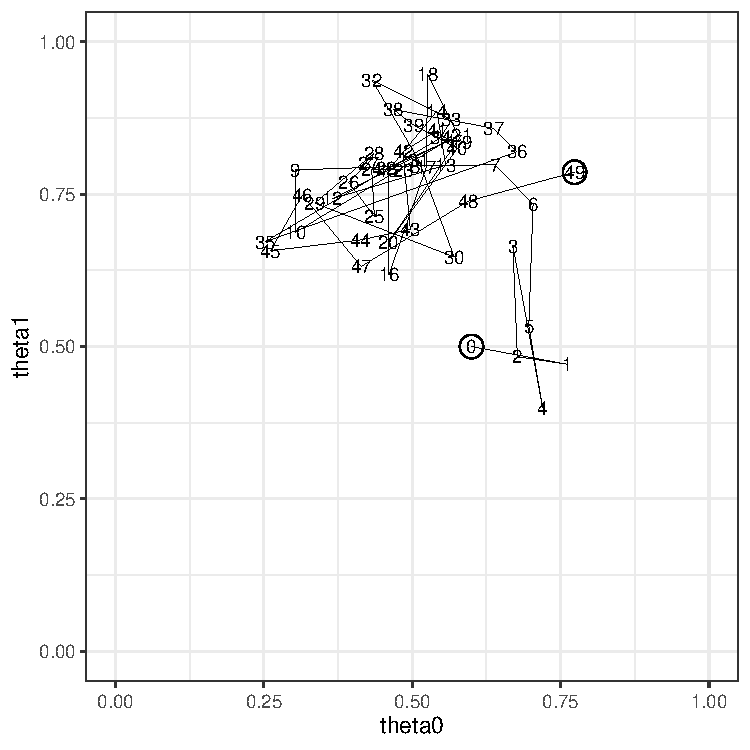
\includegraphics[page=1,keepaspectratio,width=\textwidth]{./source/ip_figure1.pdf}
\end{center}
\normalsize
\end{column}
\end{columns}
\end{frame}

\begin{frame}[label={sec:org549b92f}]{Visual Representation of Posterior Samples}
\begin{columns}
\begin{column}{0.50\columnwidth}
\begin{itemize}
\item 10\textsuperscript{4} posterior samples were obtained.
\item The first 10\% of posterior samples were discarded to reduce the influence of the initialization values.
\end{itemize}
\end{column}

\begin{column}{0.50\columnwidth}
\scriptsize
\begin{center}
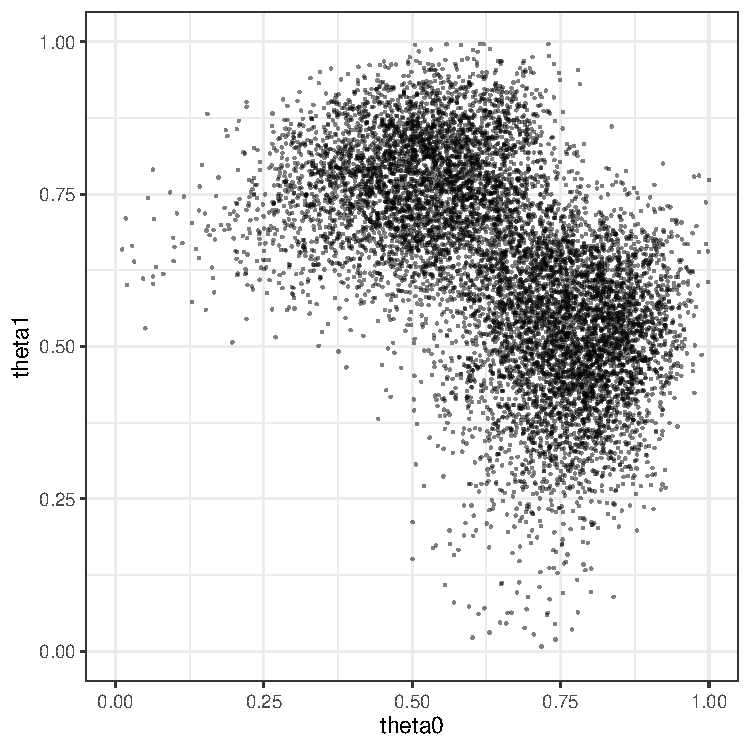
\includegraphics[page=1,keepaspectratio,width=\textwidth]{./source/ip_figure2.pdf}
\end{center}
\normalsize
\end{column}
\end{columns}
\end{frame}

\begin{frame}[label={sec:org7bf486b}]{Visual Representation of Posterior Density}
\begin{columns}
\begin{column}{0.50\columnwidth}
\begin{itemize}
\item The first 10\% of posterior samples were discarded to reduce the influence of the initialization values.
\item Similarly to the EM results with multiple initialization values, the posterior exhibits bimodality.
\end{itemize}
\end{column}

\begin{column}{0.50\columnwidth}
\scriptsize
\begin{center}
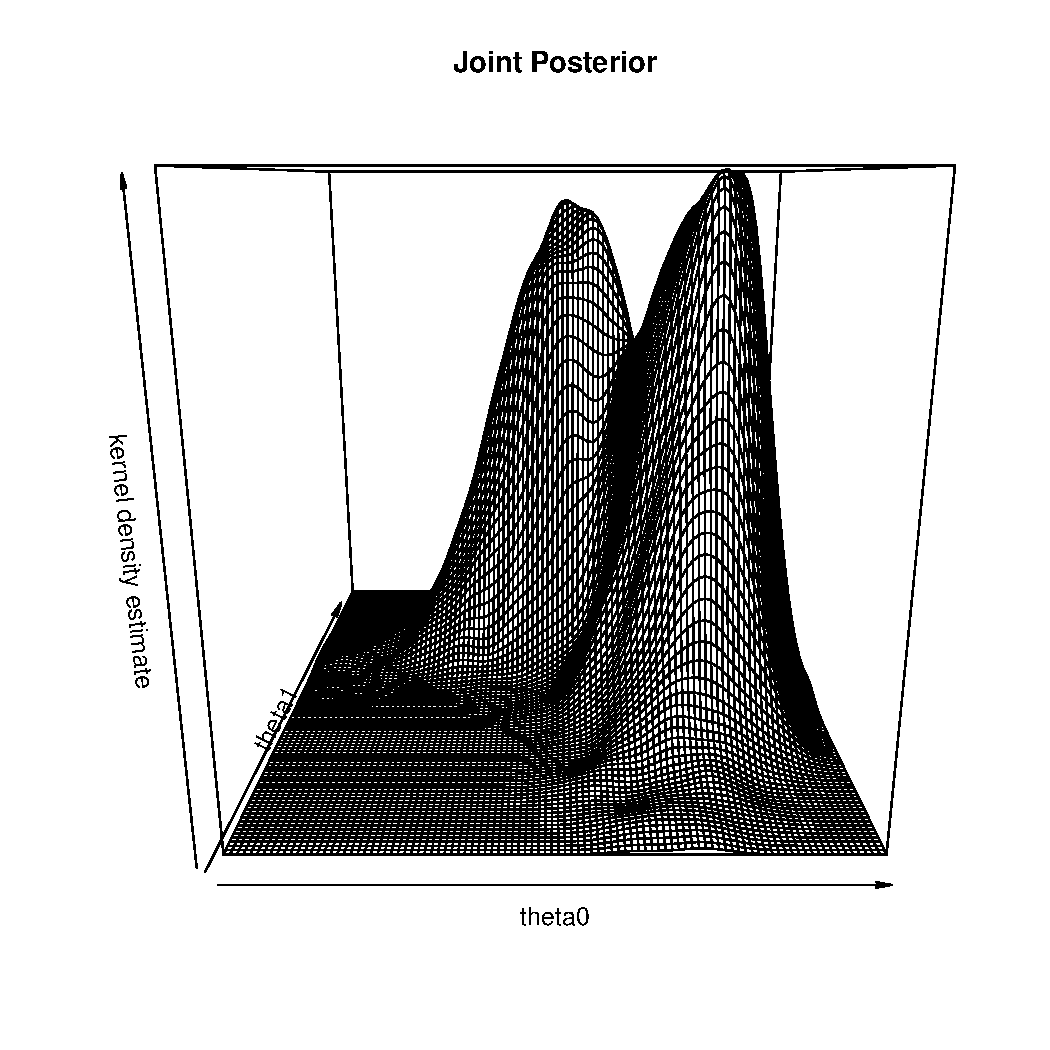
\includegraphics[page=1,keepaspectratio,width=\textwidth]{./source/ip_figure3.pdf}
\end{center}
\normalsize
\end{column}
\end{columns}
\end{frame}

\begin{frame}[label={sec:orgd6b65e3}]{DA: Animation}
\begin{columns}
\begin{column}{0.50\columnwidth}
\begin{itemize}
\item Incomplete-data likelihood function.
\item \href{https://github.com/kaz-yos/em\_da\_repo/blob/master/source/ip\_rgl.gif}{Animated gif on Github}
\item Note that the marginalized posterior and tentative posteriors are not drawn to the scale.
\end{itemize}
\end{column}

\begin{column}{0.50\columnwidth}
\begin{center}
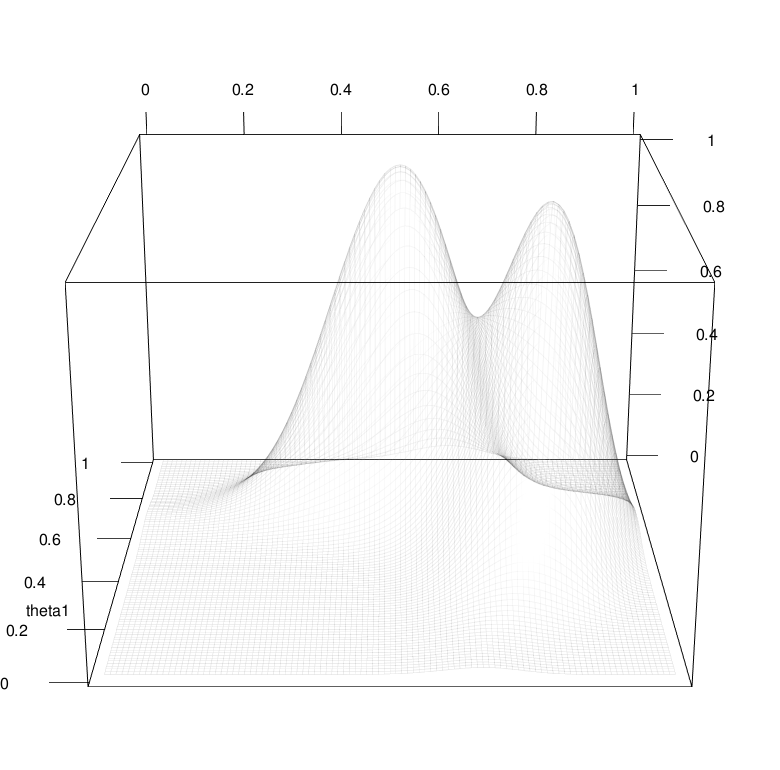
\includegraphics[page=1,keepaspectratio,width=\textwidth,height=\textheight]{./source/ip_rgl_.png}
\end{center}
\end{column}
\end{columns}
\end{frame}

\section{Stan}
\label{sec:org6e2589f}
\appendix
\begin{frame}[label={sec:org2303ea5}]{}
\begin{center}
\resizebox{\linewidth}{!}{Sampling Using Stan}
\end{center}
\end{frame}

\begin{frame}[label={sec:orgc1a264f}]{Stan: Hamiltonian Monte Carlo}
\begin{itemize}
\item Traditional Bayesian posterior sampling software, such as WinBUGS \cite{lunnWinBUGSBayesianModelling2000} and JAGS \cite{plummerJAGSProgramAnalysis2003}, are Gibbs samplers.
\item Gibbs sampling in this incomplete-data setting implements the data augmentation method.
\item Stan \cite{carpenterStanProbabilisticProgramming2017} is a modern Bayesian posterior sampler, which uses more efficient joint posterior sampling scheme based on Hamiltonian Monte Carlo (HMC) \cite{betancourtConceptualIntroductionHamiltonian2017}.
\item However, HMC cannot handle discrete parameters, so the latent state have to be integrated (summed) out of the posterior (marginal posterior). \cite{standevelopmentteamStanUserGuide2019} (Chapter 7) \cite{lambertStudentGuideBayesian2018} (Chapters 16 and 19.4)
\item This is very similar to the EM algorithm, which uses the marginal likelihood.
\end{itemize}
\end{frame}

\begin{frame}[allowframebreaks,label=,t]{Marginalized Posterior Derivation}
\begin{itemize}
\item We are interested in the posterior distribution of the parameters given the observed data only.
\end{itemize}
\begin{align*}
  &~~~\text{Introduce latent state}\\
  p(\btheta | \bX)
  &= \sum_{\bz} p(\btheta, \bz | \bX)\\
  &= \sum^{1}_{z_{1}=0}\dots\sum^{1}_{z_{5}=0} p(\btheta, z_{1},\dots,z_{5} | \bX_{1},\dots,\bX_{5})\\
  &~~~\text{Bayes rule}\\
  &\propto \sum^{1}_{z_{1}=0}\dots\sum^{1}_{z_{5}=0} p(\btheta, z_{1},\dots,z_{5}, \bX_{1},\dots,\bX_{5})\\
  &~~~\text{iid given parameter}\\
  &= \sum^{1}_{z_{1}=0}\dots\sum^{1}_{z_{5}=0} \prod^{5}_{i=1}p(X_{i} | z_{i},\btheta) p(z_{i}) p(\btheta)\\
  % https://math.stackexchange.com/questions/705945/how-to-interchange-a-sum-and-a-product
  &= \prod^{5}_{i=1} \sum^{1}_{z_{i}=0} p(X_{i} | z_{i},\btheta) p(z_{i}) p(\btheta)\\
  &= p(\btheta) \prod^{5}_{i=1} \sum^{1}_{z_{i}=0} p(X_{i} | z_{i},\btheta) p(z_{i})\\
  &= p(\btheta) \prod^{5}_{i=1} \sum^{1}_{z_{i}=0} p(X_{i} | z_{i}, \btheta) (0.5)\\
  &\propto p(\btheta) \prod^{5}_{i=1} \sum^{1}_{z_{i}=0} p(X_{i} | z_{i}, \btheta)
\end{align*}
\end{frame}

\begin{frame}[fragile,allowframebreaks,label=,t]{Stan Implementation}
 \begin{itemize}
\item The marginalized posterior expression can be implemented as follows in the Stan language.
\end{itemize}
\scriptsize
\begin{minted}[frame=lines,linenos=false]{r}
stan_code <- readr::read_file("./coin.stan")
cat(stan_code)
\end{minted}

\begin{verbatim}

/* Stan Code */
data {
    real<lower=0> a[2];
    real<lower=0> b[2];
    int<lower=0> N;
    int<lower=0> X[N];
}

parameters {
    real<lower=0,upper=1> theta[2];
}

model {
    /* Prior's contribution to posterior log probability. */
    for (i in 1:2) {
        target += beta_lpdf(theta[i] | a[i], b[i]);
    }
    /* Data (likelihood)'s contribution to posterior log probability. */
    for (i in 1:N) {
        /* This part sums out the latent coin identity. */
        target += log_sum_exp(binomial_lpmf(X[i] | 10, theta[1]),
                              binomial_lpmf(X[i] | 10, theta[2]));
    }
}
\end{verbatim}

\normalsize
\scriptsize
\normalsize
\newpage
\begin{itemize}
\item Printing the model object gives a summary.
\end{itemize}
\scriptsize
\begin{verbatim}
Inference for Stan model: 4d47aa8560f5c81f88fd6a3e63af7988.
12 chains, each with iter=10000; warmup=5000; thin=1; 
post-warmup draws per chain=5000, total post-warmup draws=60000.

           mean se_mean   sd   2.5%    25%    50%   75% 97.5% n_eff Rhat
theta[1]   0.64    0.00 0.17   0.29   0.51   0.65  0.77  0.92 12103    1
theta[2]   0.64    0.00 0.17   0.29   0.52   0.66  0.77  0.91 12097    1
lp__     -10.43    0.01 1.08 -13.43 -10.76 -10.05 -9.73 -9.51 14398    1

Samples were drawn using NUTS(diag_e) at Mon Apr 15 07:04:07 2019.
For each parameter, n_eff is a crude measure of effective sample size,
and Rhat is the potential scale reduction factor on split chains (at 
convergence, Rhat=1).
\end{verbatim}

\normalsize
\end{frame}

\begin{frame}[label={sec:orgcbb353f}]{Stan Diagnostic Plots}
\begin{columns}
\begin{column}{0.50\columnwidth}
\begin{center}
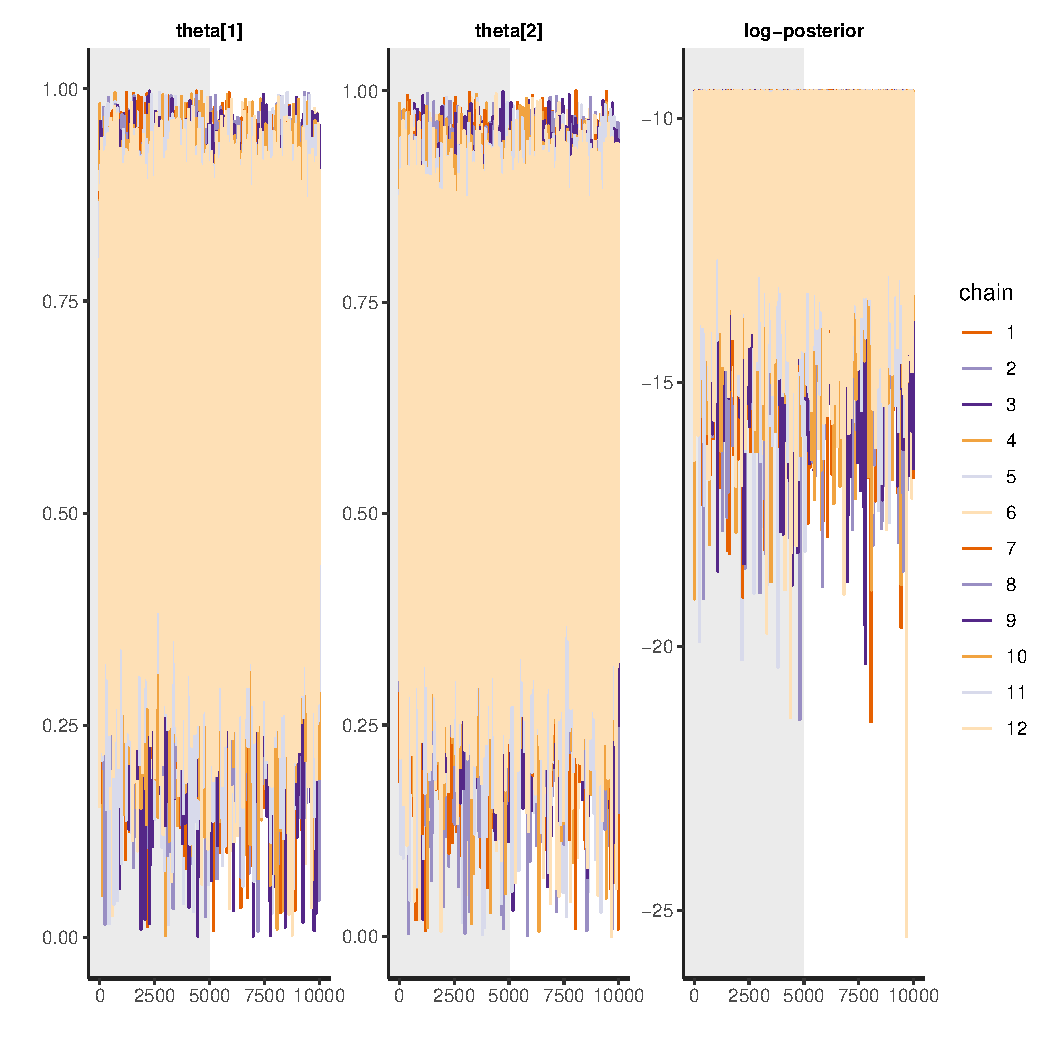
\includegraphics[page=1,keepaspectratio,width=\textwidth,height=\textheight]{./source/figure_stan_trace.pdf}
\end{center}
\normalsize
\end{column}

\begin{column}{0.50\columnwidth}
\scriptsize
\begin{center}
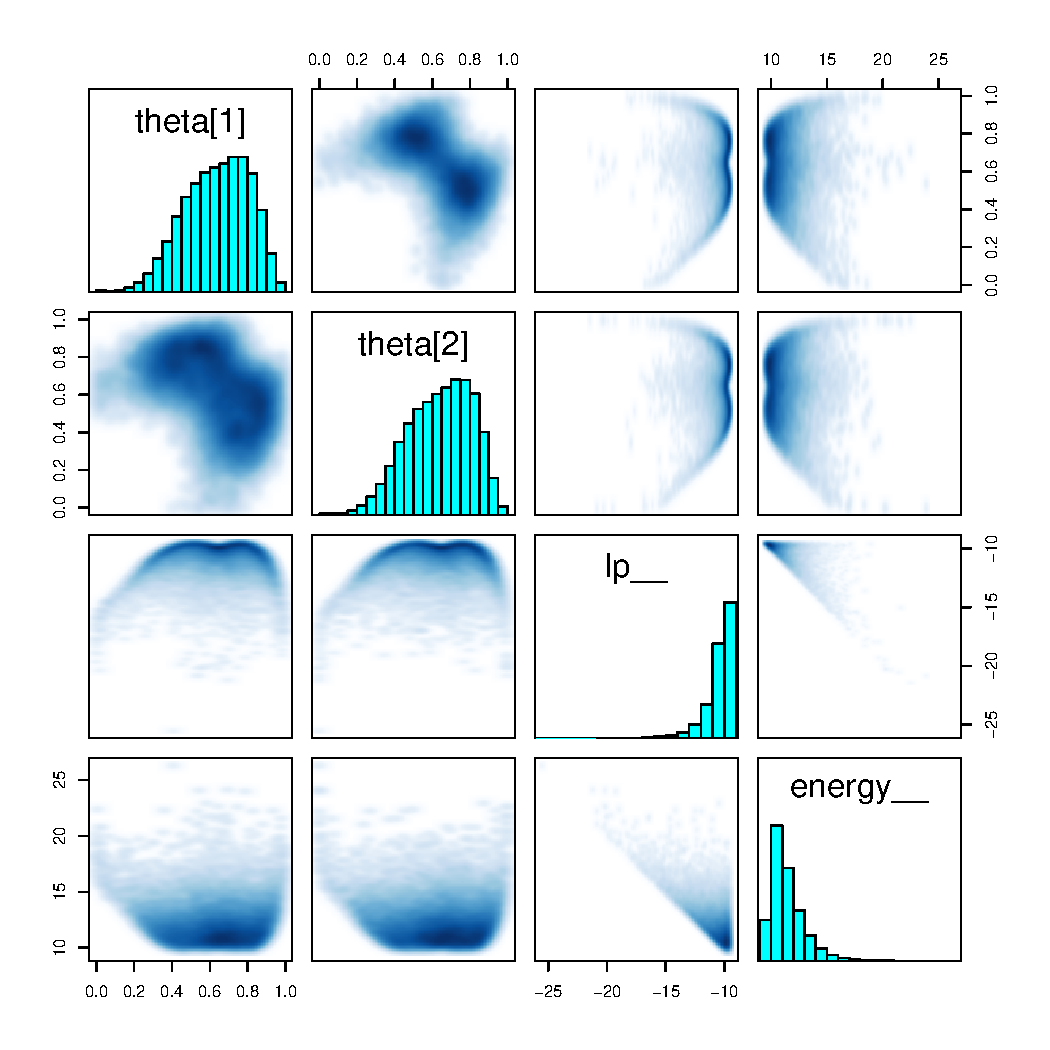
\includegraphics[page=1,keepaspectratio,width=\textwidth,height=\textheight]{./source/figure_stan_pairs.pdf}
\end{center}
\normalsize
\end{column}
\end{columns}
\end{frame}

\begin{frame}[label={sec:orgcb16f8c}]{Visual Representation of Stan Initial Iterations}
\begin{columns}
\begin{column}{0.50\columnwidth}
\begin{itemize}
\item Duplicated points are rejected HMC proposal
\end{itemize}
\end{column}

\begin{column}{0.50\columnwidth}
\scriptsize
\begin{center}
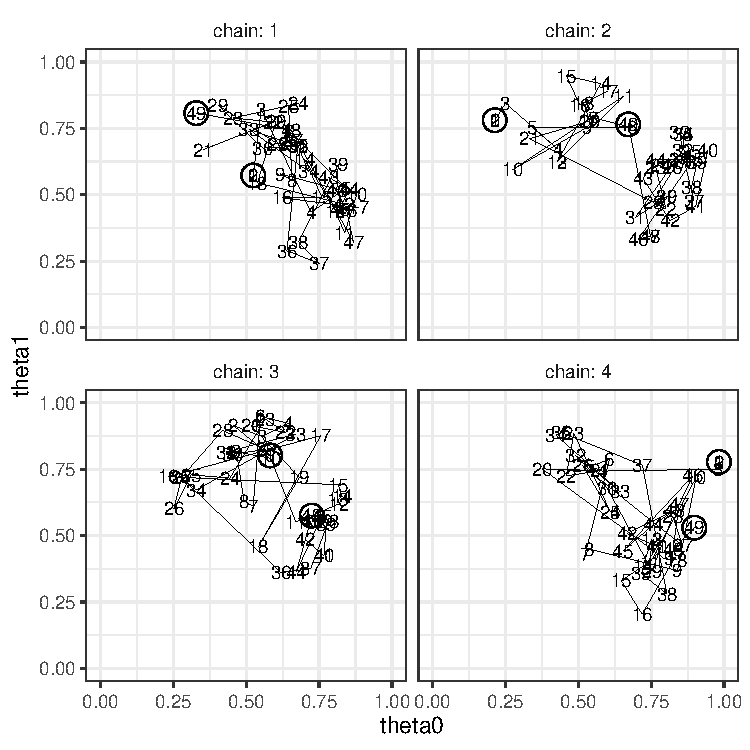
\includegraphics[page=1,keepaspectratio,width=\textwidth]{./source/figure_stan_init.pdf}
\end{center}
\normalsize
\end{column}
\end{columns}
\end{frame}

\begin{frame}[label={sec:org984b819}]{Stan Posterior Samples}
\begin{columns}
\begin{column}{0.50\columnwidth}
\begin{itemize}
\item The posterior distribution is essentially the same as the data augmentation version.
\item The same bimodality issue persists.
\item However, quantities that do not refer to a specific component like the posterior predictive for a new observation have no issue. \cite{standevelopmentteamStanUserGuide2019} (Chapter 5.5)
\end{itemize}
\end{column}

\begin{column}{0.50\columnwidth}
\scriptsize
\begin{center}
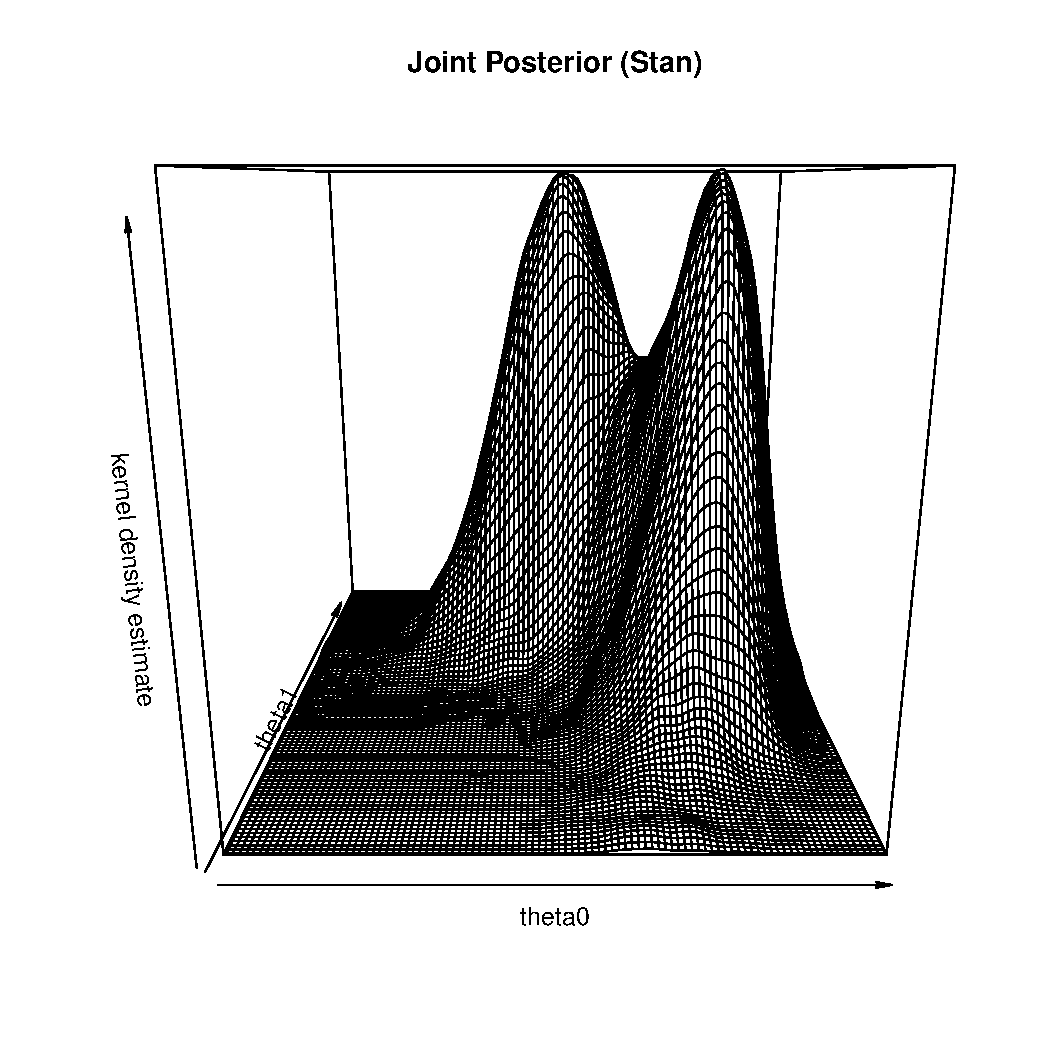
\includegraphics[page=1,keepaspectratio,width=\textwidth,height=\textheight]{./source/figure_stan.pdf}
\end{center}
\normalsize
\end{column}
\end{columns}
\end{frame}

\begin{frame}[fragile,allowframebreaks,label=,t]{Stan Implementation (Ordered Prior)}
 \begin{itemize}
\item We can avoid the indeterminancy (bimodality) by restricting the prior such that \(\theta_{0} \le \theta_{1}\) with probability 1, which in turn restricts the posterior.
\item This approach required some tricks as explained in the Stan code.
\end{itemize}
\scriptsize
\begin{minted}[frame=lines,linenos=false]{r}
stan_code_ordered <- readr::read_file("./coin_ordered.stan")
cat(stan_code_ordered)
\end{minted}

\begin{verbatim}

/* Stan Code */
data {
    real<lower=0> a[2];
    real<lower=0> b[2];
    int<lower=0> N;
    int<lower=0> X[N];
}

parameters {
    /* ordered cannot be directly used with <lower=0,upper=1> */
    /* https://groups.google.com/forum/#!topic/stan-users/7r02EU7mL3o */
    /* https://mc-stan.org/docs/2_19/stan-users-guide/reparameterizations.html */
    /* This means that HMC works with the density function for log_odds_theta? */
    ordered[2] log_odds_theta;
}

transformed parameters {
    real<lower=0,upper=1> theta[2];
    for (j in 1:2) {
        theta[j] = inv_logit(log_odds_theta[j]);
    }
}

model {
    /* Prior's contribution to posterior log probability. */
    for (j in 1:2) {
        /* Need for Jacobian adjustment */
        /* http://rpubs.com/kaz_yos/stan_jacobian */
        /*  */
        /* We have to make the distribution of log_odss_theta (eta here) contribute. */
        /* Let eta = log(theta / (1 - theta)) */
        /* theta = e^eta / (1 + e^eta) = expit(eta) */
        /* Check: https://www.wolframalpha.com/input/?i=e%5Ex+%2F+(1+%2Be%5Ex) */
        /* d theta / d eta = d expit(eta) / d eta = e^eta / (1 + e^eta)^2 */
        /* f_eta(eta) = f_theta(expit(eta)) * |d expit(eta) / d eta| */
        /*            = f_theta(theta) * (e^eta / (1 + e^eta)^2) */
        /*  */
        /* log density contributions */
        /* log f_theta(theta) can be evaluated using beta_lpdf */
        /* log (e^eta / (1 + e^eta)^2) = eta - 2 * log(1 + e^eta) */
        /*  */
        /* Beta part */
        target += beta_lpdf(theta[j] | a[j], b[j]);
        /* Jacobian part */
        target += log_odds_theta[j] - 2 * log(1 + exp(log_odds_theta[j]));
    }
    /*  */
    /* Data (likelihood)'s contribution to posterior log probability. */
    for (i in 1:N) {
        /* This part sums out the latent coin identity. */
        target += log_sum_exp(binomial_lpmf(X[i] | 10, theta[1]),
                              binomial_lpmf(X[i] | 10, theta[2]));
    }
}
\end{verbatim}

\normalsize
\scriptsize
\normalsize
\scriptsize
\begin{verbatim}
Inference for Stan model: 3bf7e32cefa48a5bf3972056c564adbb.
12 chains, each with iter=10000; warmup=5000; thin=1; 
post-warmup draws per chain=5000, total post-warmup draws=60000.

                    mean se_mean   sd   2.5%    25%    50%   75% 97.5% n_eff
log_odds_theta[1]   0.03    0.00 0.50  -1.07  -0.28   0.07  0.38  0.90 11743
log_odds_theta[2]   1.30    0.00 0.60   0.37   0.89   1.23  1.63  2.69 35238
theta[1]            0.51    0.00 0.12   0.25   0.43   0.52  0.59  0.71 12335
theta[2]            0.77    0.00 0.09   0.59   0.71   0.77  0.84  0.94 32297
lp__              -10.41    0.01 1.15 -13.47 -10.91 -10.06 -9.56 -9.24 12808
                  Rhat
log_odds_theta[1]    1
log_odds_theta[2]    1
theta[1]             1
theta[2]             1
lp__                 1

Samples were drawn using NUTS(diag_e) at Mon Apr 15 07:05:02 2019.
For each parameter, n_eff is a crude measure of effective sample size,
and Rhat is the potential scale reduction factor on split chains (at 
convergence, Rhat=1).
\end{verbatim}

\normalsize
\end{frame}

\begin{frame}[label={sec:orgcb00eb3}]{Stan Diagnostic Plots (Ordered Prior)}
\begin{columns}
\begin{column}{0.50\columnwidth}
\begin{center}
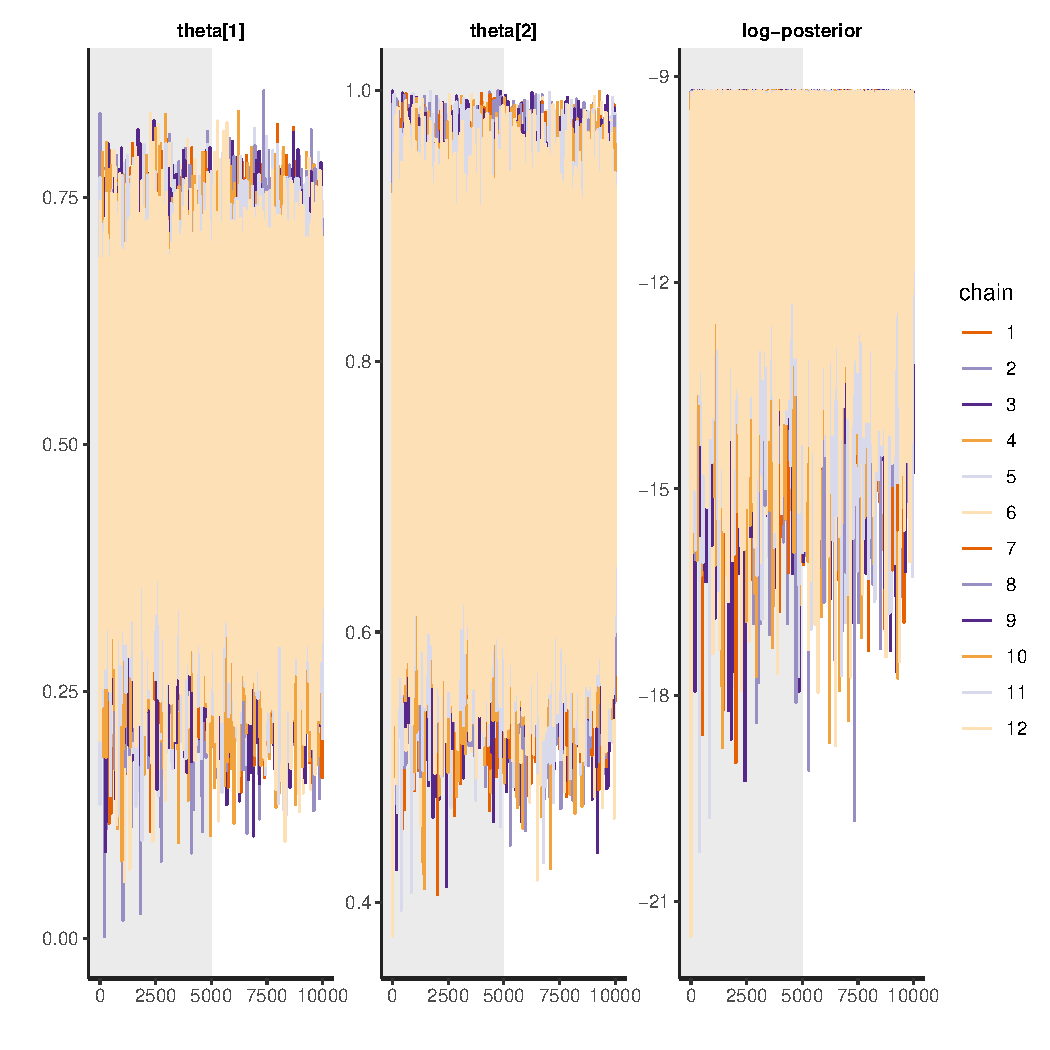
\includegraphics[page=1,keepaspectratio,width=\textwidth,height=\textheight]{./source/figure_stan_trace_ordered.pdf}
\end{center}
\normalsize
\end{column}

\begin{column}{0.50\columnwidth}
\scriptsize
\begin{center}
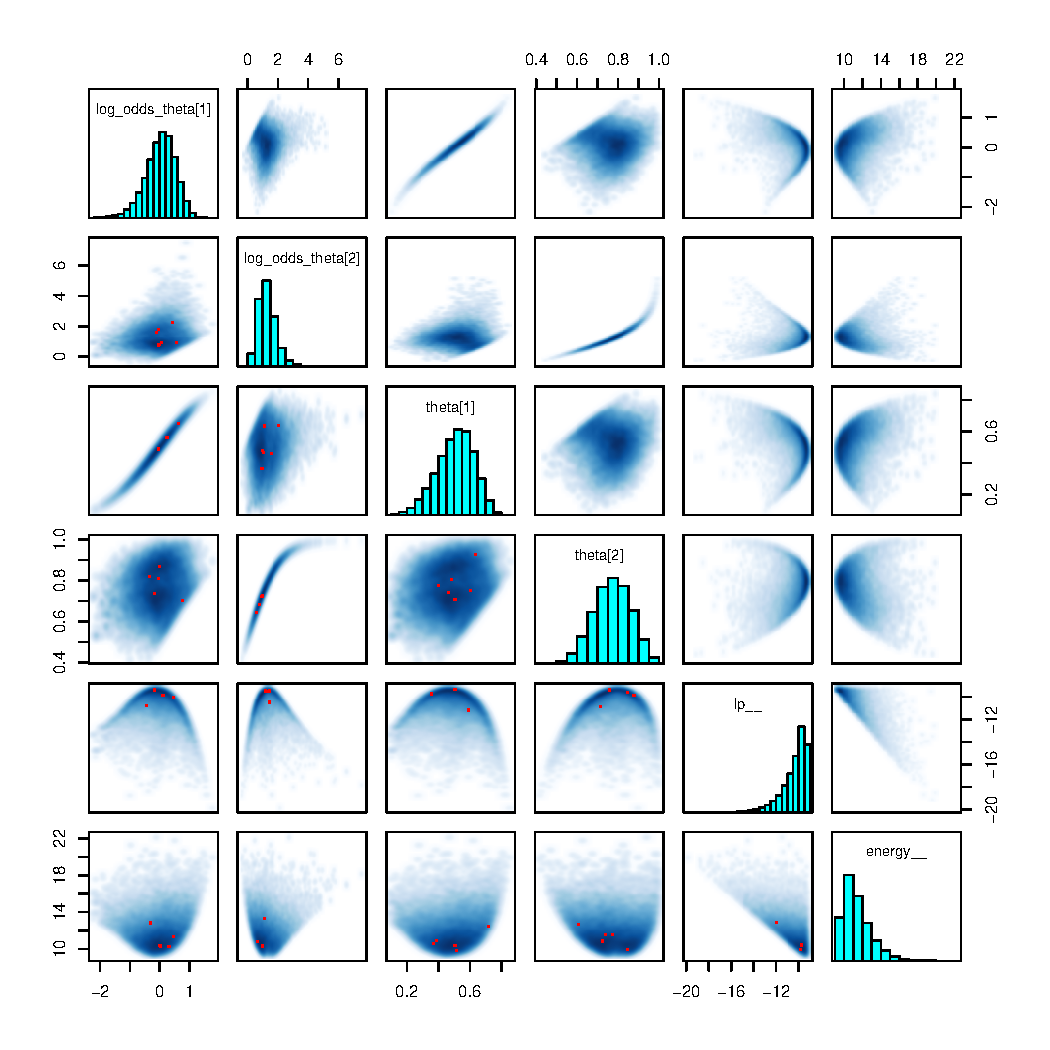
\includegraphics[page=1,keepaspectratio,width=\textwidth,height=\textheight]{./source/figure_stan_pairs_ordered.pdf}
\end{center}
\normalsize
\end{column}
\end{columns}
\end{frame}

\begin{frame}[label={sec:org8092f0d}]{Visual Representation of Stan Initial Iterations (Ordered Prior)}
\begin{columns}
\begin{column}{0.50\columnwidth}
\begin{itemize}
\item The lower diagonal part is ruled out by the prior, so the chains only wander around the upper diagonal space.
\end{itemize}
\end{column}

\begin{column}{0.50\columnwidth}
\scriptsize
\begin{center}
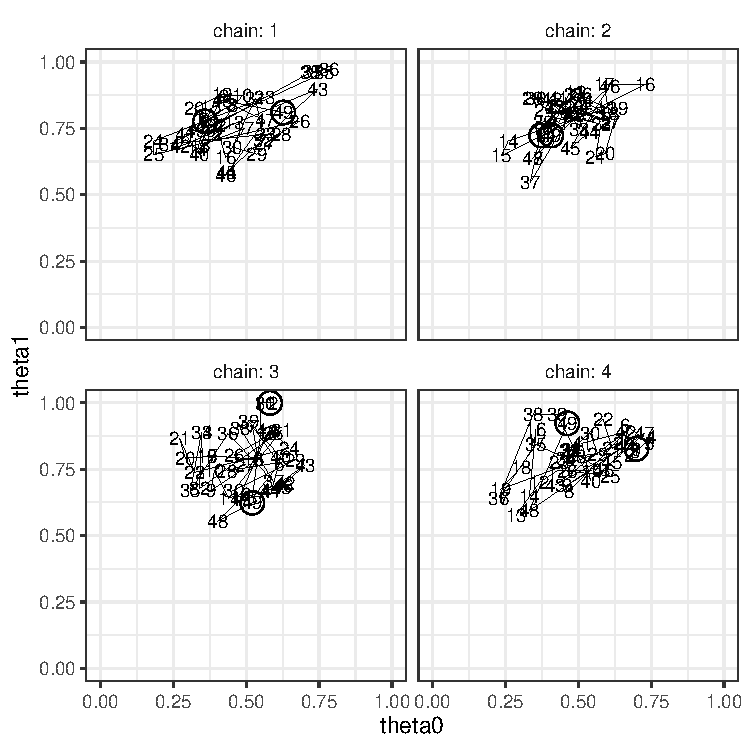
\includegraphics[page=1,keepaspectratio,width=\textwidth]{./source/figure_stan_init_ordered.pdf}
\end{center}
\normalsize
\end{column}
\end{columns}
\end{frame}

\begin{frame}[label={sec:org88e18f5}]{Stan Posterior Samples (Ordered Prior)}
\begin{columns}
\begin{column}{0.50\columnwidth}
\begin{itemize}
\item We have a unimodal posterior as we effectively banned the lower diagonal mode previously seen.
\end{itemize}
\end{column}

\begin{column}{0.50\columnwidth}
\scriptsize
\begin{center}
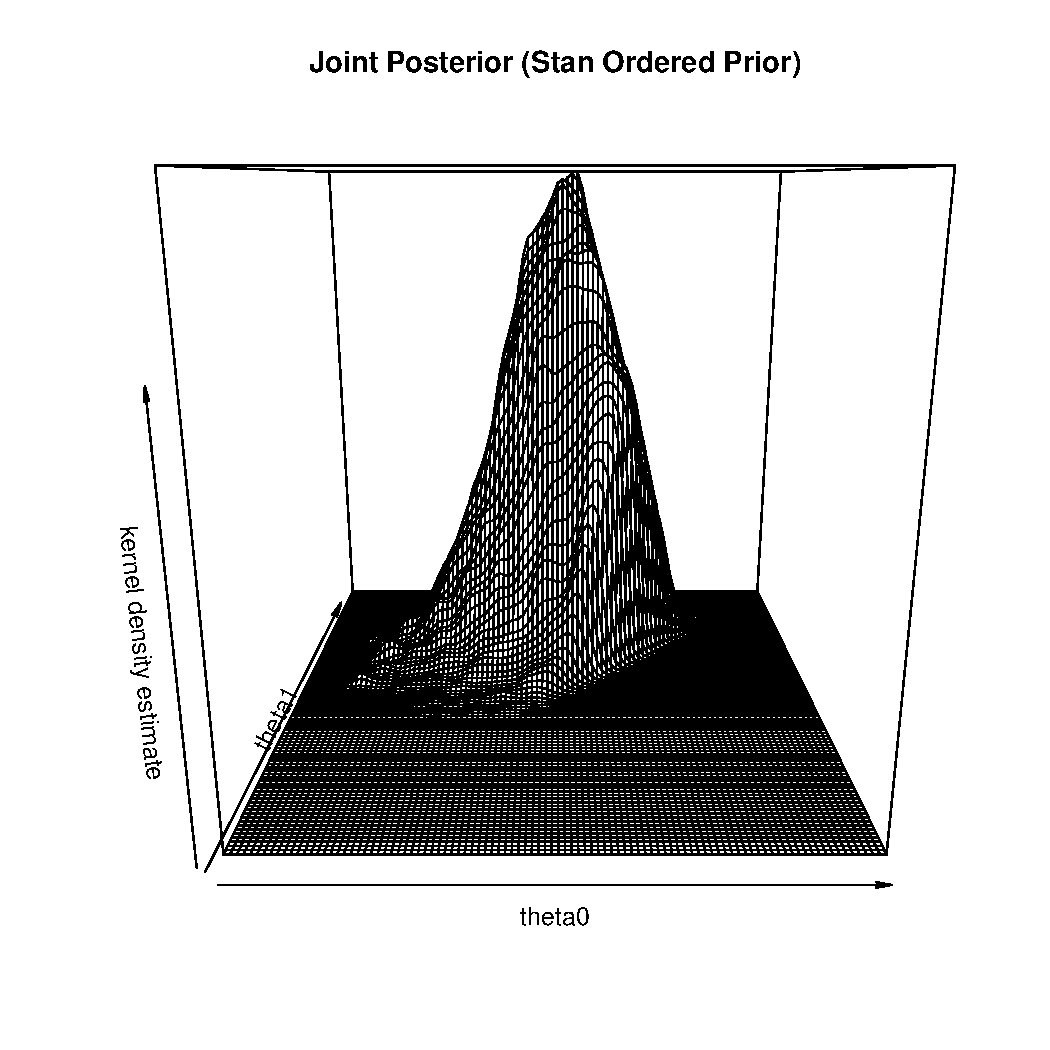
\includegraphics[page=1,keepaspectratio,width=\textwidth,height=\textheight]{./source/figure_stan_ordered.pdf}
\end{center}
\normalsize
\end{column}
\end{columns}
\end{frame}

\section{Appendix}
\label{sec:org5fae506}
\appendix
\begin{frame}[allowframebreaks,label=,t]{Bibliography}
\tiny

\renewcommand{\section}[2]{}

\bibliographystyle{apalike}
\bibliography{../../../../.emacs.d/misc/zotero}
\end{frame}
\end{document}